\documentclass[a4paper]{article}

\def\npart {III}
\def\nterm {Michaelmas}
\def\nyear {2017}
\def\nlecturer {P. Sousi}
\def\ncourse {Percolation and Random Walks on Graphs}
\def\nofficial {http://www.statslab.cam.ac.uk/~ps422/percolation.html}
% Imports
\ifx \nextra \undefined
  \usepackage[pdftex,
    hidelinks,
    pdfauthor={Dexter Chua},
    pdfsubject={Cambridge Maths Notes: Part \npart\ - \ncourse},
    pdftitle={Part \npart\ - \ncourse},
  pdfkeywords={Cambridge Mathematics Maths Math \npart\ \nterm\ \nyear\ \ncourse}]{hyperref}
  \title{Part \npart\ - \ncourse}
\else
  \usepackage[pdftex,
    hidelinks,
    pdfauthor={Dexter Chua},
    pdfsubject={Cambridge Maths Notes: Part \npart\ - \ncourse\ (\nextra)},
    pdftitle={Part \npart\ - \ncourse\ (\nextra)},
  pdfkeywords={Cambridge Mathematics Maths Math \npart\ \nterm\ \nyear\ \ncourse\ \nextra}]{hyperref}

  \title{Part \npart\ - \ncourse \\ {\Large \nextra}}
\fi

\author{Lectured by \nlecturer \\\small Notes taken by Dexter Chua}
\date{\nterm\ \nyear}

\usepackage{alltt}
\usepackage{amsfonts}
\usepackage{amsmath}
\usepackage{amssymb}
\usepackage{amsthm}
\usepackage{booktabs}
\usepackage{caption}
\usepackage{enumitem}
\usepackage{fancyhdr}
\usepackage{graphicx}
\usepackage{mathtools}
\usepackage{microtype}
\usepackage{multirow}
\usepackage{pdflscape}
\usepackage{pgfplots}
\usepackage{siunitx}
\usepackage{tabularx}
\usepackage{tikz}
\usepackage{tkz-euclide}
\usepackage[normalem]{ulem}
\usepackage[all]{xy}

\pgfplotsset{compat=1.12}

\pagestyle{fancyplain}
\lhead{\emph{\nouppercase{\leftmark}}}
\ifx \nextra \undefined
  \rhead{
    \ifnum\thepage=1
    \else
      \npart\ \ncourse
    \fi}
\else
  \rhead{
    \ifnum\thepage=1
    \else
      \npart\ \ncourse\ (\nextra)
    \fi}
\fi
\usetikzlibrary{arrows}
\usetikzlibrary{decorations.markings}
\usetikzlibrary{decorations.pathmorphing}
\usetikzlibrary{positioning}
\usetikzlibrary{fadings}
\usetikzlibrary{intersections}
\usetikzlibrary{cd}

\newcommand*{\Cdot}{\raisebox{-0.25ex}{\scalebox{1.5}{$\cdot$}}}
\newcommand {\pd}[2][ ]{
  \ifx #1 { }
    \frac{\partial}{\partial #2}
  \else
    \frac{\partial^{#1}}{\partial #2^{#1}}
  \fi
}

% Theorems
\theoremstyle{definition}
\newtheorem*{aim}{Aim}
\newtheorem*{axiom}{Axiom}
\newtheorem*{claim}{Claim}
\newtheorem*{cor}{Corollary}
\newtheorem*{defi}{Definition}
\newtheorem*{eg}{Example}
\newtheorem*{fact}{Fact}
\newtheorem*{law}{Law}
\newtheorem*{lemma}{Lemma}
\newtheorem*{notation}{Notation}
\newtheorem*{prop}{Proposition}
\newtheorem*{thm}{Theorem}

\renewcommand{\labelitemi}{--}
\renewcommand{\labelitemii}{$\circ$}
\renewcommand{\labelenumi}{(\roman{*})}

\let\stdsection\section
\renewcommand\section{\newpage\stdsection}

% Strike through
\def\st{\bgroup \ULdepth=-.55ex \ULset}

% Maths symbols
\newcommand{\bra}{\langle}
\newcommand{\ket}{\rangle}

\newcommand{\N}{\mathbb{N}}
\newcommand{\Z}{\mathbb{Z}}
\newcommand{\Q}{\mathbb{Q}}
\renewcommand{\H}{\mathbb{H}}
\newcommand{\R}{\mathbb{R}}
\newcommand{\C}{\mathbb{C}}
\newcommand{\Prob}{\mathbb{P}}
\renewcommand{\P}{\mathbb{P}}
\newcommand{\E}{\mathbb{E}}
\newcommand{\F}{\mathbb{F}}
\newcommand{\cU}{\mathcal{U}}
\newcommand{\RP}{\mathbb{RP}}
\newcommand{\CP}{\mathbb{CP}}

\newcommand{\ph}{\,\cdot\,}

\DeclareMathOperator{\sech}{sech}
\DeclareMathOperator{\cosech}{cosech}
\DeclareMathOperator{\cosec}{cosec}

\DeclareMathOperator{\covol}{covol}
\DeclareMathOperator{\vol}{vol}

\let\Im\relax
\let\Re\relax
\DeclareMathOperator{\Im}{Im}
\DeclareMathOperator{\Re}{Re}
\DeclareMathOperator{\im}{im}
\DeclareMathOperator{\image}{image}
\DeclareMathOperator{\Ann}{Ann}

\DeclareMathOperator*{\res}{res}
\DeclareMathOperator{\Res}{Res}
\DeclareMathOperator{\Ind}{Ind}

\DeclareMathOperator{\tr}{tr}
\DeclareMathOperator{\diag}{diag}
\DeclareMathOperator{\rank}{rank}
\DeclareMathOperator{\card}{card}
\DeclareMathOperator{\spn}{span}
\DeclareMathOperator{\adj}{adj}

\DeclareMathOperator{\erf}{erf}
\DeclareMathOperator{\erfc}{erfc}

\DeclareMathOperator{\ord}{ord}
\DeclareMathOperator{\Sym}{Sym}

\DeclareMathOperator{\sgn}{sgn}
\DeclareMathOperator{\orb}{orb}
\DeclareMathOperator{\stab}{stab}
\DeclareMathOperator{\ccl}{ccl}

\DeclareMathOperator{\lcm}{lcm}
\DeclareMathOperator{\hcf}{hcf}

\DeclareMathOperator{\Int}{Int}
\DeclareMathOperator{\id}{id}

\DeclareMathOperator{\betaD}{beta}
\DeclareMathOperator{\gammaD}{gamma}
\DeclareMathOperator{\Poisson}{Poisson}
\DeclareMathOperator{\binomial}{binomial}
\DeclareMathOperator{\multinomial}{multinomial}
\DeclareMathOperator{\Bernoulli}{Bernoulli}
\DeclareMathOperator{\like}{like}

\DeclareMathOperator{\var}{var}
\DeclareMathOperator{\cov}{cov}
\DeclareMathOperator{\bias}{bias}
\DeclareMathOperator{\mse}{mse}
\DeclareMathOperator{\corr}{corr}

\DeclareMathOperator{\otp}{otp}
\DeclareMathOperator{\dom}{dom}

\DeclareMathOperator{\Root}{Root}
\DeclareMathOperator{\supp}{supp}
\DeclareMathOperator{\rel}{rel}
\DeclareMathOperator{\Hom}{Hom}
\DeclareMathOperator{\Aut}{Aut}
\DeclareMathOperator{\Gal}{Gal}
\DeclareMathOperator{\Mat}{Mat}
\DeclareMathOperator{\End}{End}
\DeclareMathOperator{\Char}{char}
\DeclareMathOperator{\ev}{ev}
\DeclareMathOperator{\St}{St}
\DeclareMathOperator{\Lk}{Lk}
\DeclareMathOperator{\disc}{disc}
\DeclareMathOperator{\Isom}{Isom}
\DeclareMathOperator{\length}{length}
\DeclareMathOperator{\energy}{energy}
\DeclareMathOperator{\area}{area}
\DeclareMathOperator{\Syl}{Syl}
\DeclareMathOperator{\cl}{cl}
\DeclareMathOperator{\fix}{fix}

\newcommand{\GL}{\mathrm{GL}}
\newcommand{\SL}{\mathrm{SL}}
\newcommand{\PGL}{\mathrm{PGL}}
\newcommand{\PSL}{\mathrm{PSL}}
\newcommand{\PSU}{\mathrm{PSU}}
\newcommand{\Or}{\mathrm{O}}
\newcommand{\SO}{\mathrm{SO}}
\newcommand{\U}{\mathrm{U}}
\newcommand{\SU}{\mathrm{SU}}

\renewcommand{\d}{\mathrm{d}}
\newcommand{\D}{\mathrm{D}}

\tikzset{->/.style = {decoration={markings,
                                  mark=at position 1 with {\arrow[scale=2]{latex'}}},
                      postaction={decorate}}}
\tikzset{<-/.style = {decoration={markings,
                                  mark=at position 0 with {\arrowreversed[scale=2]{latex'}}},
                      postaction={decorate}}}
\tikzset{<->/.style = {decoration={markings,
                                   mark=at position 0 with {\arrowreversed[scale=2]{latex'}},
                                   mark=at position 1 with {\arrow[scale=2]{latex'}}},
                       postaction={decorate}}}
\tikzset{->-/.style = {decoration={markings,
                                   mark=at position #1 with {\arrow[scale=2]{latex'}}},
                       postaction={decorate}}}
\tikzset{-<-/.style = {decoration={markings,
                                   mark=at position #1 with {\arrowreversed[scale=2]{latex'}}},
                       postaction={decorate}}}

\tikzset{circ/.style = {fill, circle, inner sep = 0, minimum size = 3}}
\tikzset{mstate/.style={circle, draw, blue, text=black, minimum width=0.7cm}}

\definecolor{mblue}{rgb}{0.2, 0.3, 0.8}
\definecolor{morange}{rgb}{1, 0.5, 0}
\definecolor{mgreen}{rgb}{0.1, 0.4, 0.2}
\definecolor{mred}{rgb}{0.5, 0, 0}

\def\drawcirculararc(#1,#2)(#3,#4)(#5,#6){%
    \pgfmathsetmacro\cA{(#1*#1+#2*#2-#3*#3-#4*#4)/2}%
    \pgfmathsetmacro\cB{(#1*#1+#2*#2-#5*#5-#6*#6)/2}%
    \pgfmathsetmacro\cy{(\cB*(#1-#3)-\cA*(#1-#5))/%
                        ((#2-#6)*(#1-#3)-(#2-#4)*(#1-#5))}%
    \pgfmathsetmacro\cx{(\cA-\cy*(#2-#4))/(#1-#3)}%
    \pgfmathsetmacro\cr{sqrt((#1-\cx)*(#1-\cx)+(#2-\cy)*(#2-\cy))}%
    \pgfmathsetmacro\cA{atan2(#2-\cy,#1-\cx)}%
    \pgfmathsetmacro\cB{atan2(#6-\cy,#5-\cx)}%
    \pgfmathparse{\cB<\cA}%
    \ifnum\pgfmathresult=1
        \pgfmathsetmacro\cB{\cB+360}%
    \fi
    \draw (#1,#2) arc (\cA:\cB:\cr);%
}
\newcommand\getCoord[3]{\newdimen{#1}\newdimen{#2}\pgfextractx{#1}{\pgfpointanchor{#3}{center}}\pgfextracty{#2}{\pgfpointanchor{#3}{center}}}

\def\Xint#1{\mathchoice
   {\XXint\displaystyle\textstyle{#1}}%
   {\XXint\textstyle\scriptstyle{#1}}%
   {\XXint\scriptstyle\scriptscriptstyle{#1}}%
   {\XXint\scriptscriptstyle\scriptscriptstyle{#1}}%
   \!\int}
\def\XXint#1#2#3{{\setbox0=\hbox{$#1{#2#3}{\int}$}
     \vcenter{\hbox{$#2#3$}}\kern-.5\wd0}}
\def\ddashint{\Xint=}
\def\dashint{\Xint-}


\let\div\relax
\DeclareMathOperator\div{div}

\renewcommand\L{\mathbb{L}}
\newcommand\Pci[1]{\P_{#1}(|\mathcal{C}(0)| = \infty)}
\begin{document}
\maketitle
{\small
\setlength{\parindent}{0em}
\setlength{\parskip}{1em}

A phase transition means that a system undergoes a radical change when a continuous parameter passes through a critical value. We encounter such a transition every day when we boil water. The simplest mathematical model for phase transition is percolation. Percolation has a reputation as a source of beautiful mathematical problems that are simple to state but seem to require new techniques for a solution, and a number of such problems remain very much alive. Amongst connections of topical importance are the relationships to so-called Schramm--Loewner evolutions (SLE), and to other models from statistical physics. The basic theory of percolation will be described in this course with some emphasis on areas for future development.

Our other major topic includes random walks on graphs and their intimate connection to electrical networks; the resulting discrete potential theory has strong connections with classical potential theory. We will develop tools to determine transience and recurrence of random walks on infinite graphs. Other topics include the study of spanning trees of connected graphs. We will present two remarkable algorithms to generate a uniform spanning tree (UST) in a finite graph $G$ via random walks, one due to Aldous-Broder and another due to Wilson. These algorithms can be used to prove an important property of uniform spanning trees discovered by Kirchhoff in the 19th century: the probability that an edge is contained in the UST of $G$, equals the effective resistance between the endpoints of that edge.

\subsubsection*{Pre-requisites}
There are no essential pre-requisites beyond probability and analysis at undergraduate levels, but a familiarity with the measure-theoretic basis of probability will be helpful.
}
\tableofcontents

\setcounter{section}{-1}
\section{Introduction}
This course is naturally divided into two parts --- percolation, and random walks on graphs. Percolation is one of the simplest models that experience phase transition --- an abrupt change in quantitative feature due to a continuous change of a parameter. More sophisticated examples of percolation the boiling of water and the loss of long-range correlation in magnets when temperature increases.

But we are not physicists. So let's talk about percolation. For reasons that become clear later, consider an $n \times (n + 1)$ lattice connected by edges:
\begin{center}
  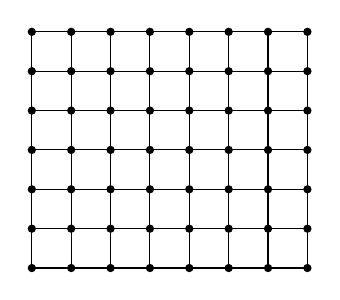
\begin{tikzpicture}[scale=0.5]
    \draw (0, 0) rectangle (7, 6);
    \foreach \x in {1,2,3,4,5,6}{
      \draw (\x, 0) -- (\x, 6);
      \draw (0, \x) -- (7, \x);
    }
    \draw (7, 0) -- (7, 6);
    \foreach \x in {0,...,7}{
      \foreach \y in {0,...,6}{
        \node [circ] at (\x, \y) {};
      }
    }
  \end{tikzpicture}
\end{center}
We now fix some $p \in [0, 1]$, and for each edge in the graph, we either keep it or remove it with probability $p$. There are many questions we may ask. For example, we may ask for the probability that there is a left-to-right crossing of open edges.
\begin{center}
  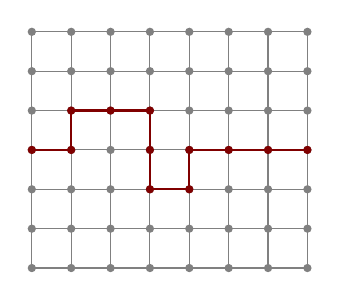
\begin{tikzpicture}[scale=0.5]
    \draw [gray] (0, 0) rectangle (7, 6);
    \foreach \x in {1,2,3,4,5,6}{
      \draw [gray] (\x, 0) -- (\x, 6);
      \draw [gray] (0, \x) -- (7, \x);
    }
    \draw [gray] (7, 0) -- (7, 6);
    \foreach \x in {0,...,7}{
      \foreach \y in {0,...,6}{
        \node [gray, circ] at (\x, \y) {};
      }
    }
    \draw [thick, mred] (0, 3) node [circ] {} -- (1, 3) node [circ] {} -- (1, 4) node [circ] {} -- (2, 4) node [circ] {} -- (3, 4) node [circ] {} -- (3, 3) node [circ] {} -- (3, 2) node [circ] {} -- (4, 2) node [circ] {} -- (4, 3) node [circ] {} -- (5, 3) node [circ] {} -- (6, 3) node [circ] {} -- (7, 3) node [circ] {};
  \end{tikzpicture}
\end{center}
For example, we have $f_n(0) = 0$ and $f_n(1) = 1$.

An interesting choice of $p$ to consider is $p = \frac{1}{2}$. We can argue that $f_n(\frac{1}{2})$ must be $\frac{1}{2}$, by symmetry. More precisely, consider the dual lattice:
\begin{center}
  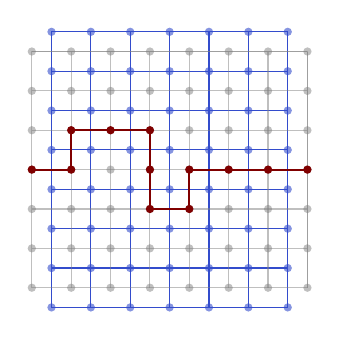
\begin{tikzpicture}[scale=0.5]
    \draw [mblue] (0.5, -0.5) rectangle (6.5, 6.5);
    \foreach \x in {1,2,3,4,5,6}{
      \draw [mblue] (\x-0.5, -0.5) -- (\x - 0.5, 6.5);
      \draw [mblue] (0.5, \x - 0.5) -- (6.5, \x - 0.5);
    }

    \draw [gray, opacity=0.5] (0, 0) rectangle (7, 6);
    \foreach \x in {1,2,3,4,5,6}{
      \draw [gray, opacity=0.5] (\x, 0) -- (\x, 6);
      \draw [gray, opacity=0.5] (0, \x) -- (7, \x);
    }
    \draw [gray, opacity=0.5] (7, 0) -- (7, 6);
    \foreach \x in {0,...,7}{
      \foreach \y in {0,...,6}{
        \node [gray, circ, opacity=0.5] at (\x, \y) {};
      }
    }

    \foreach \x in {0,...,7}{
      \foreach \y in {0,...,6}{
        \node [mblue, opacity=0.6, circ] at (\y + 0.5, \x - 0.5) {};
      }
    }

    \draw [thick, mred] (0, 3) node [circ] {} -- (1, 3) node [circ] {} -- (1, 4) node [circ] {} -- (2, 4) node [circ] {} -- (3, 4) node [circ] {} -- (3, 3) node [circ] {} -- (3, 2) node [circ] {} -- (4, 2) node [circ] {} -- (4, 3) node [circ] {} -- (5, 3) node [circ] {} -- (6, 3) node [circ] {} -- (7, 3) node [circ] {};
  \end{tikzpicture}
\end{center}
Note that this lattice is isomorphic to the original lattice we were thinking about, by applying a rotation. Now each edge in the dual lattice crosses exactly one edge in the original lattice, and we can set the edge to be open iff the corresponding edge in the original lattice is open. This gives rise to a percolation on the dual lattice with $p = \frac{1}{2}$ as well.

Now notice that that there is a left-right crossing of open edges in the original lattice iff there is no top-bottom crossing in the dual graph. But since the dual and original lattices are isomorphic, it follows that the probability that there is a left-right crossing in the original lattice is equal to the probability that there is \emph{no} left-right crossing in the original lattice. So both of these must be $\frac{1}{2}$.

The ability to talk about the dual graph is a very important property that is only true in $2$ dimensions. In general, there are many things known for $2$ dimensions via the dual, which do not generalize to higher dimensions.

The other topic we are going to discuss is random walks in graphs. In IB Markov chains, and maybe IA Probability, we considered random walks on the integer lattice $\Z^d$. Here we shall consider random walks on \emph{any graph}. We shall mostly think about finite graphs, but we will also talk about how certain results can be extended to infinite graphs. It turns out a rather useful way of thinking about this is to think of the graph as representing an electrical network. Then many concepts familiar from high school physics translate to interesting properties about the graph, and importing well-known (and elementary) results from electrical networks helps us understand graphs better.

\section{Percolation}
\subsection{The critical probability}
There are two models of percolation --- \term{bond percolation} and \term{site percolation}. In this course, we will focus on bond percolation, but we will look at site percolation in the example sheets.

The very basic set up of percolation theory involves picking a \term{graph} $G = (V, E)$, where \term{$V$} is the set of \term{vertices} and \term{$E$} is the set of \term{edges}. We also pick a \term{percolation probability} $p \in [0, 1]$. For each edge $e \in E$, we keep it with probability $p$ and throw it with probability $1 - p$. In the first case, we say the edge is \emph{open}\index{open edge}\index{edge!open}, and in the latter, we say it is \emph{closed}\index{closed edge}\index{edge!closed}.

More precisely, we define the probability space to be $\Omega= \{0, 1\}^E$, where $0$ denotes a closed edge and $1$ denotes an open one (in the case of site percolation, we have $\Omega = \{0, 1\}^V$). We endow $\Omega$ with the $\sigma$-algebra generated by \term{cylinder sets}
\[
  \{\omega \in \Omega: \omega(e) = x_e \text{ for all }e \in A\},
\]
where $A$ is a finite set and $x_e \in \{0, 1\}$ for all $e$. In other words, this is the product $\sigma$-algebra. As probability measure, we take the product measure $\P_p$, i.e.\ every edge is $1$ with probability $p$ and $0$ with probability $1 - p$. We will write \index{$\eta_p$}$\eta_p \in \{0, 1\}^E$ for the state of the system.

Now what can we say about the graph resulting from this process? One question we may ask is whether we can connect two points in the graphs via the edges that remain. To further the discussion, we introduce some notation.

\begin{notation}
  We write \term{$x \leftrightarrow y$} if there is an open path of edges from $x$ to $y$.
\end{notation}

\begin{notation}
  We write $\mathcal{C}(x) = \{y \in V: y \leftrightarrow x\}$\index{$\mathcal{C}(x)$}, the \term{cluster} of $x$.
\end{notation}

\begin{notation}
  We write $x \leftrightarrow \infty$ if $|\mathcal{C}(x)| = \infty$.
\end{notation}

From now on, we shall take $G = \L^d = (\Z^d, E(\Z^d))$, the $d$-dimensional integer lattice.\index{$\L^d$} Then by translation invariance, $|\mathcal{C}(x)|$ has the same distribution as $|\mathcal{C}(0)|$ for all $x$. We now introduce a key piece of notation:
\begin{defi}[$\theta(p)$]\index{$\theta_p$}
  We define $\theta(p) = \P_p(|\mathcal{C}(0)| = \infty)$.
\end{defi}

Most of the questions we ask surround this $\theta(p)$. We first make the most elementary observations:
\begin{eg}
  $\theta(0) = 0$ and $\theta(1) = 1$.
\end{eg}

A natural question to ask is then if we can find $p \in (0, 1)$ such that $\theta(p) > 0$. But even before answering that question, we can ask a more elementary one --- is $\theta$ an increasing function of $p$?

Intuitively, it must be. And we can prove it. The proof strategy is known as \term{coupling}. We have already seen coupling in IB Markov Chains, where we used it to prove the convergence to the invariant distribution under suitable conditions. Here we are going to couple all percolation processes for different values of $P$.

\begin{lemma}
  $\theta$ is an increasing function of $p$.
\end{lemma}

\begin{proof}
  We let $(U(e))_{e \in E(\Z^d)}$ be iid $U[0, 1]$ random variables. For each $p \in [0, 1]$, we define
  \[
    \eta_p(e) =
    \begin{cases}
      1 & U(e) \leq p\\
      0 & \text{otherwise}
    \end{cases}
  \]
  Then $\P(\eta_p(e) = 1) = \P(U(e) < p) = p$. Since the $U(e)$ are independent, so are $\eta_p$. Thus $\eta_p$ has the law of bond percolation with probability $p$.

  Moreover, if $p \leq q$, then $\eta_p(e) \leq \eta_q(e)$. So the result follows.
\end{proof}
Note that this is not only useful as a theoretical tool. If we want to simulate percolation with different probabilities $p$, we can simply generate a set of $U[0, 1]$ variables, and use it to produce a percolation for all $p$.

If we wish, we can provide an abstract definition of what coupling is, but the detailed definition is not of much practical use:
\begin{defi}[Coupling]\index{coupling}
  Let $\mu$ and $\nu$ be two probability measures on (potentially) different probability spaces. A \emph{coupling} is a pair of random variables $(X, Y)$ defined on the same probability space such that the marginal distribution of $X$ is $\mu$ and the marginal distribution of $Y$ is $\nu$.
\end{defi}

%The obvious first question to ask is then:
%\begin{question}
%  Is there $p \in (0, 1)$ such that $\theta(p) > 0$?
%\end{question}
%
%In the degenerate case $d = 1$, we immediately see that we have
%\begin{eg}
%  Take $d = 1$. Then for any $p < 1$, we have $\theta(p) = 0$.
%\end{eg}
%
%If $\theta(p)$ is not always zero, then there is an immediate follow-up question we can ask:
%\begin{question}
%  Is $\theta(p)$ increasing?
%\end{question}
%Intuitively, this must be the case, and indeed we will show that it is true.
%
%Finally, a questions we can ask is:
%\begin{question}
%  Suppose $\theta(p) > 0$. Then how many infinite components are there?
%\end{question}
%
%We first answer question $2$. What we are going to use is \emph{coupling}. The definition will look a little abstract, but we will use it a lot, and we shall see how it is useful in practice.

With the lemma, we can make the definition
\begin{defi}[Critical probability]\index{Critical probability}
  We define $p_c(d) = \sup \{p \in [0, 1]: \theta(p) = 0\}$.
\end{defi}

Recall we initially asked whether $\theta(p)$ can be non-zero for $p \in (0, 1)$. We can now rephrase and strengthen this question by asking for the value of $p_c(d)$. There are a lot more questions we can ask about $p_c$ and $\theta(p)$.

For example, we know that $\theta(p)$ is a $C^\infty$ function on $(p_c, 1]$. However, we do not know if $\theta$ is continuous at $p_c$ in $d = 3$. We will see soon that $p_c = \frac{1}{2}$ in $d = 2$, but the exact value of $p_c$ is not known in higher dimensions.

Let's start actually proving things about $p_c$. We previously noted that
\begin{prop}
  $p_c(1) = 1$.
\end{prop}

The first actually interesting theorem is the following:
\begin{thm}
  For all $d \geq 2$, we have $p_c(d) \in (0, 1)$.
\end{thm}

We shall break this up into two natural parts:
\begin{lemma}
  For $d \geq 2$, $p_c(d) > 0$.
\end{lemma}

\begin{proof}
  Write $\Sigma_n$ for the number of open self-avoiding paths of length $n$ starting at $0$. We then note that
  \[
    \P_p(|\mathcal{C}(0)| = \infty) = \P_p(\forall n \geq 1: \Sigma_n \geq 1) = \lim_{n \to \infty} \P_p(\Sigma_n \geq 1) \leq \lim_{n \to \infty} \E_p[\Sigma_n].
  \]
  We can now compute $\E_p[\Sigma_n]$. The point is that expectation is linear, which makes this much easier to compute. We let $\sigma_n$ be the number of self-avoiding paths\index{self-avoiding paths} of length $n$ from $0$. Then we simply have
  \[
    \E_p[\Sigma_n] = \sigma_n p^n.
  \]
  We can bound $\sigma_n$ by $2d \cdot (2d - 1)^{n - 1}$, since we have $2d$ choices of the first step, and at most $2d - 1$ choices in each subsequent step. So we have
  \[
    \E_p[\Sigma_n] \leq 2d (2d - 1)^{n - 1} p^n = \frac{2d}{2d - 1} (p(2d - 1))^n.
  \]
  So if $p (2d - 1) < 1$, then $\theta(p) = 0$. So we know that
  \[
    p_c(d) \geq \frac{1}{2d - 1}.\qedhere
  \]
\end{proof}

Before we move on to the other half of the theorem, we talk a bit more about \term{self-avoiding paths}.
\begin{defi}[$\sigma_n$]\index{$\sigma_n$}
  We write $\sigma_n$ for the number of self-avoiding paths of length $n$ starting from $0$.
\end{defi}
In the proof, we used the rather crude bound
\[
  \sigma_n \leq 2d \cdot (2d - 1)^{n - 1}.
\]
More generally, we can make the following bound:

\begin{lemma}
  We have $\sigma_{n + m} \leq \sigma_n \sigma_m$.
\end{lemma}

\begin{proof}
  A self-avoiding path of length $n + m$ can be written as a concatenation of self-avoiding paths of length $n$ starting from $0$ and another one of length $m$.
\end{proof}
Taking the logarithm, we know that $\log \sigma_n$ is a \term{subadditive sequence}. It turns out this property alone is already quite useful. It is an exercise in analysis to prove the following lemma:

\begin{lemma}[Fekete's lemma]\index{Fekete's lemma}
  If $(a_n)$ is a subadditive sequence of real numbers, then
  \[
    \lim_{n \to \infty} \frac{a_n}{n} = \inf\left\{\frac{a_k}{k}: k \geq 1\right\} \in [-\infty, \infty).
  \]
  In particular, the limit exists.
\end{lemma}

This allows us to define
\begin{defi}[$\lambda$ and $\kappa$]\index{$\lambda$}\index{$\kappa$}
  We define
  \[
    \lambda = \lim_{n \to \infty} \frac{\log \sigma_n}{n},\quad \kappa = e^\lambda.
  \]
  $\kappa$ is known as the \term{connective constant}.
\end{defi}

Then by definition, we have
\[
  \sigma_n= e^{n \lambda (1 + o(1))} = \kappa^{n + o(n)}.
\]
as $n \to \infty$.

Thus, asymptotically, the growth rate of $\sigma_n$ is determined by $\kappa$. It is natural to then seek for the value of $\kappa$, but unfortunately we don't know the value of $\kappa$ for the Euclidean lattice. A bit more on the positive side, the value for the hexagonal lattice has been found recently:
\begin{thm}[Duminil-Copin, Smirnov, 2010]
  The hexagonal lattice has
  \[
    \kappa_{\mathrm{hex}} = \sqrt{2 + \sqrt{2}}.
  \]
\end{thm}

We might want to be a bit more precise about how $\sigma_n$ grows. For $d \geq 5$, we have the following theorem:
\begin{thm}[Hara and Slade, 1991]
  For $d \geq 5$, there exists a constant $A$ such that
  \[
    \sigma_n = A \kappa^n (1 + O(n^{-\varepsilon}))
  \]
  for any $\varepsilon < \frac{1}{2}$.
\end{thm}

We don't really know what happens when $d < 5$, but we have the following conjecture:

\begin{conjecture}
  \[
    \sigma_n \approx
    \begin{cases}
      n^{11/32} \kappa^n & d = 2\\
      n^\gamma \kappa^n & d = 3\\
      (\log n)^{1/4} \kappa^n & d = 4
    \end{cases}
  \]
\end{conjecture}

One can also instead try to bound $\sigma_n$ from above. We have the following classic theorem:
\begin{thm}[Hammersley and Welsh, 1962]
  For all $d \geq 2$, we have
  \[
    \sigma_n \leq C \kappa^n \exp(c' \sqrt{n})
  \]
  for some constants $C$ and $c'$.
\end{thm}

In fact, a better bound was recently found:
\begin{thm}[Hutchcroft, 2017]
  For $d \geq 2$, we have
  \[
     \sigma_n \leq C \kappa^n \exp(o(\sqrt{n})).
  \]
\end{thm}
This will be proved in the example sheet.

What would be a good way to understand self-avoiding walks? Fixing an $n$, there are only finitely many self-avoiding walks of length $n$. So we can sample such a self-avoiding walk uniformly at random. In general, we would expect the total displacement of the walk to be $\sim \sqrt{n}$. Thus, what we can try to do is to take $n \to \infty$ while simultaneously shrinking space by a factor of $\frac{1}{\sqrt{n}}$. We would then hope that the result converges toward some Brownian motion-like trajectory. If we can characterize the precise behaviour of this \term{scaling limit}, then we might be able to say something concrete about $\kappa$ and the asymptotic behaviour of $\sigma_n$.

But we don't really know what the scaling limit is. In the case $d = 2$, it is conjectured to be $SLE(\frac{8}{3})$. Curiously, it was proven by Gwynne and Miller in 2016 that if we instead looked at self-avoiding walks on a \emph{random surface}, then the scaling limit is $SLE(\frac{8}{3})$.

That's enough of a digression. Let's finish our proof and show that $p_c(d) < 1$. A first observation is that it suffices to show this for $d = 2$. Indeed, since $\Z^d$ embeds into $\Z^{d + 1}$ for all $d$, if we can find an infinite cluster in $\Z^d$, then the same is true for $\Z^{d + 1}$. Thus, it is natural to restrict to the case of $d = 2$, where \emph{duality} will be prove to be an extremely useful tool.

\begin{defi}[Planar graph]\index{planar graph}\index{graph!planar}
  A graph $G$ is called planar if it can be embedded on the plane in such a way that no two edges cross.
\end{defi}

\begin{defi}[Dual graph]\index{dual graph}\index{graph!dual}
  Let $G$ be a planar graph (which we call the \term{primal graph}\index{graph!primal}). We define the \emph{dual graph} by placing a vertex in each face of $G$, and connecting $2$ vertices if their faces share a boundary edge.
\end{defi}

\begin{eg}
  The dual of $\Z^2$ is isomorphic to $\Z^2$ % insert picture
  \begin{center}
    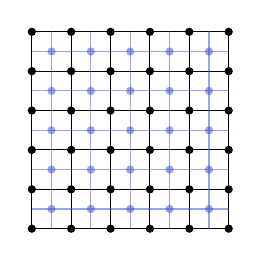
\begin{tikzpicture}[scale=0.5]
      \draw (0, 0) grid (5, 5);
      \begin{scope}[shift={(0.5, 0.5)}]
        \clip (-0.5, -0.5) rectangle (4.5, 4.5);
        \draw [mblue, opacity=0.5, step=1] (-1, -1) grid (5, 5);
      \end{scope}
      \foreach \x in {0.5, 1.5, 2.5, 3.5, 4.5} {
        \foreach \y in {0.5, 1.5, 2.5, 3.5, 4.5} {
          \node [mblue, opacity=0.5, circ] at (\x, \y) {};
        }
      }
      \foreach \x in {0, 1, 2, 3, 4, 5} {
        \foreach \y in {0, 1, 2, 3, 4, 5} {
          \node [circ] at (\x, \y) {};
        }
      }

    \end{tikzpicture}
  \end{center}
\end{eg}
The dual lattice will help us prove a lot of properties for percolation in $\Z^2$.

\begin{lemma}
  $p_c(d) < 1$ for all $d \geq 2$.
\end{lemma}

\begin{proof}
  It suffices to show this for $d = 2$. Suppose we perform percolation on $\Z^2$. Then this induces a percolation on the dual lattice by declaring an edge of the dual is open if it crosses an open edge of $\Z^2$, and closed otherwise.

  Suppose $|\mathcal{C}(0)| < \infty$ in the primal lattice. Then there is a closed circuit in the dual lattice, given by the ``boundary'' of $\mathcal{C}(0)$. Let $D_n$ be the number of closed dual circuits of length $n$ that surround $0$. Then the union bound plus Markov's inequality tells us
  \[
    \P_p(|\mathcal{C}(0)| < \infty) = \P_p(\exists n \geq D_n \geq 1) \leq \sum_{n = 4}^\infty \E_p[D_n],
  \]
  using the union bound and Markov's inequality.

  It is a simple exercise to show that
  \begin{ex}
    Show that the number of dual circuits of length $n$ that contain $0$ is at most $n \cdot 4^n$.
  \end{ex}
  From this, it follows that
  \[
    \P_p(|\mathcal{C}(0)| < \infty) \leq \sum_{n = 4}^\infty n \cdot 4^n (1 - p)^n.
  \]
  Thus, if $p$ is sufficiently near $1$, then $\P_p(|\mathcal{C}(0)| < \infty)$ is bounded away from $1$.
\end{proof}

By definition, if $p < p_c(d)$, then $0$ is almost surely not contained in an infinite cluster. If $p > p_c(d)$, then there is a positive probability that $0$ is contained in an infinite cluster. However, it is of course not necessarily the case that $0$ is connected to $\infty$ with probability $1$. In fact, there is at least probability $(1 - p)^{2d}$ that $0$ is not connected to $\infty$, since $0$ cannot be connected to $\infty$ if all its neighbouring edges are closed. However, it is still possible that there is some infinite cluster somewhere. It's just that it does not contain $0$.

\begin{prop}
  Let $A_\infty$ be the event that there is an infinite cluster.
  \begin{enumerate}
    \item If $\theta(p) = 0$, then $\P_p(A_\infty) = 0$.
    \item If $\theta(p) > 0$, then $\P_p(A_\infty) = 1$.
  \end{enumerate}
\end{prop}

\begin{proof}\leavevmode
  \begin{enumerate}
    \item We have
      \[
        \P_p(A_\infty) = \P_p(\exists x: |\mathcal{C}(x)| = \infty) \leq \sum_{x \in \Z^d} \P_p(|\mathcal{C}(x)| = \infty) = \sum \theta(p) = 0.
      \]
    \item We need to apply the \term{Kolmogorov 0-1 law}. Recall that if $X_1, X_2, \ldots$ are independent random variables, and $\mathcal{F}_n = \sigma(X_k: k \geq n)$, $\mathcal{F}_\infty = \bigcap_{n \geq 0} \mathcal{F}_n$, Then $\mathcal{F}_\infty$ is trivial, i.e.\ for all $A \in \mathcal{F}_\infty$, $\P(A) \in \{0, 1\}$.

      So we order the edges of $\Z^d$ as $e_1, e_2, \ldots$ and denote their states
      \[
        w(e_1), w(e_2), \ldots.
      \]
      These are iid random variables. We certainly have $\P_p(A_\infty) \geq \theta(p) > 0$. So if we can show that $A_\infty \in \mathcal{F}_\infty$, then we are done. But this is clear, since changing the states of a finite number of edges does not affect the occurrence of $A_\infty$.\qedhere
  \end{enumerate}
\end{proof}

The next follow up questions is how many infinite clusters do we expect to get?
\begin{thm}[Burton and Keane]
  If $p > p_c$, then there exists a unique infinite cluster with probability $1$.
\end{thm}
This proof is considerably harder than the ones we have previously done. We might think we can use the Kolmogorov 0-1 law, but we can't, since changing a finite number of edges can break up or join together infinite clusters, so the event that there are $k$ infinite clusters for $k > 0$ is not in $\mathcal{F}_\infty$. However, we can exploit the fact that $N$ is translation invariant.

\begin{ex}
  Let $A$ be an event that is translation invariant. Then $\P_p(A) = 0$ or $1$ almost surely. % prove this
\end{ex}

\begin{proof}
  Let $N$ be the number of infinite clusters. Then by the lemma, we know $N$ is constant almost surely. So there is some $k \in \N \cup \{\infty\}$ such that $\P_p(N = k) = 1$. First of all, we know that $k \not= 0$, since $\theta(p) > 0$. We shall first exclude $2 \leq k < \infty$, and then exclude $k = \infty$.

  Assume that $k < \infty$. We will show that $\P_p(n = 1) > 0$, and hence it must be the case that $\P_p(n = 1) = 1$.

  To bound this probability, we let $B(n) = [-n, n]^d \cap \Z^d$\index{$B(n)$} (which we will sometimes write as \term{$B_n$}), and let $\partial B(n)$ be its boundary. We know that
  \[
    \P_p(\text{all infinite clusters intersect $\partial B(n)$}) \to 1
  \]
  as $n \to \infty$. This is since with probability $1$, there are only finitely many clusters by assumption, and for each of these configurations, all infinite clusters intersect $\partial B(n)$ for sufficiently large $n$.

  In particular, we can take $n$ large enough such that
  \[
    \P_p(\text{all infinite clusters intersect }\partial B(n)) \geq \frac{1}{2}.
  \]
  We can then bound
  \begin{multline*}
    \P_p(N = 1) \geq \P_p(\text{all infinite clusters intersect }\partial B(n)\\
    \text{ and all edges in $B(n)$ are open}).
  \end{multline*}
  Finally, note that the two events in there are independent, since they involve different edges. But the probability that all edges in $B(n)$ are open is just $p^{E(B(n))}$. So
  \[
    \P_p(N = 1) \geq \frac{1}{2} p^{E(B(n))} > 0.
  \]
  So we are done.

  We now have to show that $k \not= \infty$. This involves the notion of a \emph{trifurcation}. The idea is that we will show that if $k = \infty$, then the probability that a vertex is a trifurcation is positive. This implies the expected number of trifurcations is $\sim n^d$. We will then show deterministically that the number of trifurcations inside $B(n)$ must be $\leq |\partial B(n)|$, and so there are $O(n^{d - 1})$ trifurcations, which is a contradiction.

  We say a vertex $x$ is a \term{trifurcation} if the following three conditions hold:
  \begin{enumerate}
    \item $x$ is in an infinite open cluster $\mathcal{C}_\infty$;
    \item There exist exactly three open edges adjacent to $x$;
    \item $\mathcal{C}_\infty \setminus \{x\}$ contains exactly three infinite clusters and no finite ones.
  \end{enumerate}
  This is clearly a translation invariant notion. So
  \[
    \P_p(0 \text{ is a trifurcation}) = \P_p(x \text{ is a trifurcation})
  \]
  for all $x \in \Z^d$.

  \begin{claim}
    $\P_p(0\text{ is a trifurcation}) > 0$.
  \end{claim}
  We need to use something slightly different from $B(n)$. We define $S(n) = \{x \in \Z^d: \|x\|_1 \leq n\}$.
  \begin{center}
    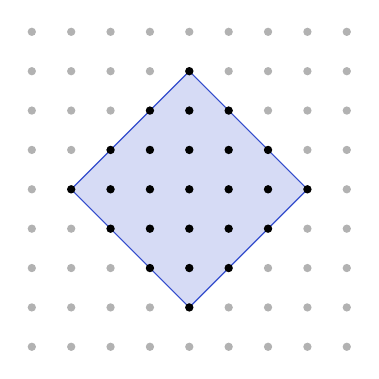
\begin{tikzpicture}[scale=0.5]
      \draw [mblue, fill opacity=0.2, fill=mblue] (-3, 0) -- (0, 3) -- (3, 0) -- (0, -3) -- cycle;
      \foreach \x in {-4,..., 4} {
        \foreach \y in {-4,..., 4} {
          \node [circ, opacity=0.3] at (\x, \y) {};
        }
      }
      \foreach \x in {-3,..., 3} {
        \pgfmathsetmacro\n{3-abs(\x)};
        \foreach \y in {-\n, ..., \n} {
          \node [circ] at (\x, \y) {};
        }
      }
    \end{tikzpicture}
  \end{center}
  The crucial property of this is that for any $x_1, x_2, x_3 \in \partial S(n)$, there exist three disjoint self-avoiding paths joining $x_i$ to $0$ (exercise!). For each triple $x_1, x_2, x_3$, we arbitrarily pick a set of three such paths, and define the event
  \begin{multline*}
    J(x_1, x_2, x_3) = \{\text{all edges on these 3 paths are open}\\\text{ and everything else inside $S(n)$ is closed}\}.
  \end{multline*}
  Next, for every possible infinite cluster in $\Z^d \setminus S(n)$ that intersects $\partial S(n)$ at at least one point, we pick a designated point of intersection arbitrarily.

  Then we can bound
  \begin{multline*}
    \P_p(0 \text{ is a trifurcation}) \geq \P_p(\exists \mathcal{C}_\infty^1, \mathcal{C}_\infty^2, \mathcal{C}_\infty^3 \subseteq \Z^d \setminus S(n)\\ \text{ infinite clusters which intersect $\partial S(n)$ at $x_1, x_2, x_3$, and $J(x_1, x_2, x_3)$}).
  \end{multline*}
  Rewrite the right-hand probability as
  \begin{multline*}
    \P_p(J(x_1, x_2, x_3) \mid\exists \mathcal{C}_\infty^1, \mathcal{C}_\infty^2, \mathcal{C}_\infty^3 \subseteq \Z\text{ intersecting }\partial S(n))\\
    \times \P_p(\exists \mathcal{C}_\infty^1, \mathcal{C}_\infty^2, \mathcal{C}_\infty^3 \subseteq \Z^d \setminus \partial S(n))
  \end{multline*}
  We can bound the first term by
  \[
    \min(p, 1 - p)^{E(S(n))}.
  \]
  To bound the second probability, we have already assumed that $\P_p(N = \infty) = 1$. So $\P_p(\exists \mathcal{C}_\infty^1, \mathcal{C}_\infty^2, \mathcal{C}_\infty^3 \subseteq \Z^d \setminus S(n)\text{ intersecting }\partial S(n)) \to 1$ as $n \to \infty$. We can then take $n$ large enough such that the probability is $\geq \frac{1}{2}$. So we have shown that $c \equiv \P_p(0\text{ is a trifurcation}) > 0$.

  Using the linearity of expectation, it follows that
  \[
    \E_p[\text{number of trifurcations inside $B(n)$})] \geq c |B(n)| \sim n^d.
  \]
  On the other hand, we can bound the number of trifurcations in $B(n)$ by $|\partial B(n)|$. To see this, suppose $x_1$ is a trifurcation in $B(n)$. By definition, there exists $3$ open paths to $\partial B(n)$. Fix three such paths. Let $x_2$ be another trifurcation. It also has $3$ open paths to the $\partial B(n)$, and its paths to the boundary could intersect those of $x_1$. However, they cannot create a cycle, by definition of a trifurcation. For simplicity, we add the rule that when we produce the paths for $x_2$, once we intersect the path of $x_1$, we continue following the path of $x_1$.

  Exploring all trifurcations this way, we obtain a forest inside $B(n)$, and the boundary points will be the leaves of the forest. Now the trifurcations have degree $3$ in this forest. The rest is just combinatorics.
  \begin{ex}
    For any tree, the number of degree $3$ vertices is always less than the number of leaves.\qedhere % prove this
  \end{ex}
\end{proof}

\subsection{Correlation inequalities}
In this section, we are going to prove some useful inequalities and equalities, and use them to prove some interesting results about $\theta(p)$ and the decay of $\P_p(0 \leftrightarrow \partial B_n)$.

To motivate our first inequality, suppose we have $4$ points $x, y, u, v$, and we want to ask for the conditional probability
\[
  \P_p(x \leftrightarrow y \mid u \leftrightarrow v).
\]
Intuitively, we expect this to be greater than $\P_p(x \leftrightarrow y)$, since $u \leftrightarrow v$ tells us there are some open edges around, which is potentially helpful. The key property underlying this intuition is that having more edges is beneficial to both of the events. To quantify this, we need the notion of an increasing random variable.

Again, let $G = (V, E)$ be a graph and $\Omega = \{0, 1\}^E$. We shall assume that $E$ is countable.

\begin{notation}[$\leq$]\index{$\leq$}
  Given $\omega, \omega' \in \Omega$, we write $\omega \leq \omega'$ if $\omega(e) \leq \omega'(e)$ for all $e \in E$.
\end{notation}
This defines a partial order on $\Omega$.

\begin{defi}[Increasing random variable]\index{increasing random variable}\index{random variable!increasing}\index{decreasing random variable}\index{random variable!decreasing}
  A random variable $X$ is increasing if $X(\omega) \leq X(\omega')$ whenever $\omega \leq \omega'$, and is decreasing if $-X$ is increasing.
\end{defi}

\begin{defi}[Increasing event]\index{increasing event}\index{event!increasing}\index{event!decreasing}\index{decreasing event}
  An event $A$ is increasing (resp.\ decreasing) if the indicator $1(A)$ is increasing (resp.\ decreasing)
\end{defi}

\begin{eg}
  $\{|\mathcal{C}(0)|= \infty\}$ is an increasing event.
\end{eg}

An immediate consequence of the definition is that
\begin{thm}
  If $N$ is an increasing random variable and $p_1 \leq p_2$, then
  \[
    \E_{p_1} [N] \leq \E_{p_2} [N],
  \]
  and if an event $A$ is increasing, then
  \[
    \P_{p_1}(A) \leq \P_{p_2}(A).
  \]
\end{thm}

\begin{proof}
  Immediate from coupling.
\end{proof}

What we want to prove is the following result, which will be extremely useful.
\begin{thm}[Fortuin--Kasteleyn--Ginibre (FKG) inequality]\index{FKG inequality}
  Let $X$ and $Y$ be increasing random variables with $\E_p[X^2], \E_p[Y^2] < \infty$. Then
  \[
    \E_p[XY] \geq \E_p[X] \E_p[Y].
  \]
  In particular, if $A$ and $B$ are increasing events, then
  \[
    \P_p(A \cap B) \geq \P_p(A) \P_p(B).
  \]
  Equivalently,
  \[
    \P_p(A \mid B) \geq \P_p(A).
  \]
\end{thm}

\begin{proof}
  The plan is to first prove this in the case where $X$ and $Y$ depend on a finite number of edges, and we do this by induction. Afterwards, the desired result can be obtained by an application of the martingale convergence theorem. In fact, the ``real work'' happens when we prove it for $X$ and $Y$ depending on a single edge. Everything else follows from messing around with conditional probabilities.

  If $X$ and $Y$ depend only on a single edge $e_1$, then for any $\omega_1, \omega_2 \in \{0, 1\}$, we claim that
  \[
    (X(\omega_1) - X(\omega_2))(Y(\omega_1) - Y(\omega_2)) \geq 0.
  \]
  Indeed, $X$ and $Y$ are both increasing. So if $\omega_1 > \omega_2$, then both terms are positive; if $\omega < \omega_2$, then both terms are negative, and there is nothing to do if they are equal.

  In particular, we have
  \[
    \sum_{\omega_1, \omega_2 \in \{0, 1\}} (X(\omega_1) - X(\omega_2)) (Y(\omega_1) - Y(\omega_2)) \P_p( \omega(e_1) = \omega_1) \P_p(\omega(e_1) = \omega_2) \geq 0.
  \]
  Expanding this, we find that the LHS is $2(\E_p[XY] - \E_p[X] \E_p[Y])$, and so we are done.

  Now suppose the claim holds for $X$ and $Y$ that depend on $n < k$ edges. We shall prove the result when they depend on $k$ edges $e_1, \ldots, e_k$. We have
  \[
    \E_p[XY] = \E_p[\E_p[XY \mid \omega(e_1), \ldots, \omega(e_{k - 1})]].
  \]
  Now after conditioning on $\omega(e_1), \ldots, \omega(e_{k - 1})$, the random variables $X$ and $Y$ become increasing random variables of $\omega(e_k)$. Applying the first step, we get
  \begin{multline*}
    \E_p[X Y \mid \omega(e_1), \ldots, \omega(e_{k - 1})]\\
    \geq \E_p[X \mid \omega(e_1), \ldots, \omega(e_{k - 1})] \E_p[Y \mid \omega(e_1), \ldots, \omega(e_{k - 1})].\tag{$*$}
  \end{multline*}
  But $\E_p[X \mid \omega(e_1), \ldots, \omega(e_{k - 1})]$ is a random variable depending on the edges $e_1, \ldots, e_{k - 1}$, and moreover it is increasing. So the induction hypothesis tells us
  \begin{multline*}
    \E_p\big[\E_p[X \mid \omega(e_1), \ldots, \omega(e_{k - 1})] \E_p[Y \mid \omega(e_1), \ldots, \omega(e_{k - 1})]\big] \\
    \geq \E_p\big[\E_p[X \mid \omega(e_1), \ldots, \omega(e_{k - 1})]\big] \E_p\big[\E_p[Y \mid \omega(e_1), \ldots, \omega(e_{k - 1})]\big]
  \end{multline*}
  Combining this with (the expectation of) ($*$) then gives the desired result.

  Finally, suppose $X$ and $Y$ depend on the states of a countable set of edges $e_1, e_2, \ldots$. Let's define
  \begin{align*}
    X_n &= \E_p [X \mid \omega(e_1), \ldots, \omega(e_n)]\\
    Y_n &= \E_p [Y \mid \omega(e_1), \ldots, \omega(e_n)]
  \end{align*}
  Then $X_n$ and $Y_n$ are martingales, and depend only on the states of only finitely many edges. So we know that
  \[
    \E_p[X_n Y_n] \geq \E_p [X_n] \E_p[Y_n] = \E_p[X] \E_p[Y].
  \]
  By the $\mathcal{L}^2$-martingale convergence theorem, $X_n \to X$, $Y_n \to Y$ in $L^2$ and almost surely. So taking the limit $n \to \infty$, we get
  \[
    \E_p[XY] \geq \E_p[X] \E_p[Y].\qedhere
  \]
\end{proof}

What we want to consider next is the notion of disjoint occurrence. For example, we want to able to ask the probability that there exists two disjoint paths connecting a pair of points.

To formulate this disjointness, suppose we have an event $A$, and let $\omega \in A$. To ask whether this occurrence of $A$ depends only on some set $S \subseteq E$ of edges, we can look at the set
\[
  [\omega]_S = \{\omega' \in \Omega: \omega'(e) = \omega(e)\text{ for all }e \in S\}.
\]
If $[\omega]_S \subseteq A$, then we can rightfully say this occurrence of $A$ depends only on the edges in $S$. Note that this depends explicitly and importantly on $\omega$, i.e.\ the ``reason'' $A$ happened. For example, if $A = \{x \leftrightarrow y\}$, and $\omega \in A$, then we can take $S$ to be the set of all edges in a chosen path from $x$ to $y$ in the configuration of $\omega$. This choice will be different for different values of $\omega$.

Using this, we can define what it means for two events to occur disjointly.
\begin{defi}[Disjoint occurrence]\index{disjoint occurrence}
  Let $F$ be a set and $\Omega = \{0, 1\}^F$. If $A$ and $B$ are events, then the event that $A$ and $B$ occurs \emph{disjointly} is
  \[
    A \circ B = \{\omega \in \Omega : \exists S \subseteq F\text{ s.t. } [\omega]_S \subseteq A \text{ and } [\omega]_{F\setminus S} \subseteq B\}.
  \]
\end{defi}

\begin{thm}[BK inequality]\index{BK inequality} % van den Berg and Kesten
  Let $F$ be a finite set and $\Omega = \{0, 1\}^F$. Let $A$ and $B$ be increasing events. Then
  \[
    \P_p(A \circ B) \leq \P_p(A) \P_p(B).
  \]
\end{thm}
This says if $A$ and $B$ are both events that ``needs'' edges to occur, then requiring that they occur disjointly is more difficult than them occurring individually.

The proof is completely magical. There exist saner proofs of the inequality, but they are rather longer.
\begin{proof}[Proof (Bollob\'as and Leader)]
  We prove by induction on the size $n$ of the set $F$. For $n = 0$, it is trivial.

  Suppose it holds for $n - 1$. We want to show it holds for $n$. For $D \subseteq \{0, 1\}^F$ and $i = 0, 1$, set
  \[
    D_i = \{(\omega_1, \ldots, \omega_{n - 1}) : (\omega_1, \ldots, \omega_{n - 1}, i) \in D\}.
  \]
  Let $A, B \subseteq \{0, 1\}^F$, and $C = A \circ B$. We check that
  \[
    C_0 = A_0 \circ B_0,\quad C_1 = (A_0 \circ B_1) \cup (A_1 \circ B_0).
  \]
  Since $A$ and $B$ are increasing, $A_0 \subseteq A_1$ and $B_0 \subseteq B_1$, and $A_i$ and $B_i$ are also increasing events. So
  \begin{align*}
    C_0 &\subseteq (A_0 \circ B_1) \cap (A_1 \circ B_0)\\
    C_1 &\subseteq A_1 \circ B_1.
  \end{align*}
  By the induction hypothesis, we have
  \begin{align*}
    \P_p(C_0) &= \P_p(A_0 \circ B_0) \leq \P_p(A_0) \P_p(B_0)\\
    \P_p(C_1) &\leq \P_p(A_1 \circ B_1) \leq \P_p(A_1) \P_p(B_1)\\
    \P_p(C_0) + \P_p(C_1) &\leq \P_p((A_0 \circ B_1) \cap (A_1 \circ B_0)) + \P_p((A \circ B_1) \cup (A_1 \circ B_0))\\
    &= \P_p(A_0 \circ B_1) + \P_p(A_1 \circ B_0)\\
    &\leq \P_p(A_0) \P_p(B_1) + \P_p(A_1) \P_p(B_0).
  \end{align*}
  Now note that for any $D$, we have
  \[
    \P_p(D) = p \P_p(D_1) + (1 - p) \P_p(D_0).
  \]
  By some black magic, we multipy the first inequality by $(1 - p)^2$, the second by $p^2$ and the third by $p(1 - p)$. This gives
  \[
    p\P_p(C_1) + (1 - p)\P_p(C_0) \leq (p\P_p(A_1) + (1- p)\P_p(A_0))(p\P_p(B_1) + (1 - p) \P_p(B_0)).
  \]
  Expand and we are done.
\end{proof}

It turns out the increasing hypothesis is not necessary:
\begin{thm}[Reimer]
  For all events $A, B$ depending on a finite set, we have $\P_p(A \circ B) \leq \P_p(A) \P_p(B)$.
\end{thm}
But the proof is much harder, and in all the case where we want to apply this, the variables are increasing.

As an application of the BK inequality, we first prove a preliminary result about the decay of $\P_p(0 \leftrightarrow \partial B(n))$. To prove our result, we will need a stronger condition than $p < p_c$. Recall that we defined
\[
  \theta(p) = \P_p( |\mathcal{C}(0)| = \infty).
\]
We also define\index{$\chi(p)$}
\[
  \chi(p) = \E_p[|\mathcal{C}(0)|].
\]
If $\chi(p)$ is finite, then of course $\theta(p) = 0$. However, the converse need not hold.

\begin{thm}
  If $\chi(p) < \infty$, then there exists a positive constant $c$ such that for all $n \geq 1$,
  \[
    \P_p(0 \leftrightarrow \partial B(n)) \leq e^{-cn}.
  \]
\end{thm}
Later, we will show that in fact this holds under the assumption that $p < p_c$. However, that requires a bit more technology, which we will develop after this proof.

The idea of the proof is that if we want a path from, say, $0$ to $B(2n)$, then the path must hit a point on $\partial B(n)$. So there is a path from $0$ to a point on $\partial B(n)$, and a path from that point to $\partial B(2n)$. Moreover, these two paths are disjoint, which allows us to apply the BK inequality.
\begin{proof}
  Let
  \[
    X_n = \sum_{x \in \partial B(n)} 1(0 \leftrightarrow x).
  \]
  Now consider
  \[
    \sum_{n = 0}^\infty \E[X_n] = \sum_n \sum_{x \in \partial B(n)} \P_p(0 \leftrightarrow x) = \sum_{x \in \Z^d} \P_p(0 \leftrightarrow x) = \chi(p).
  \]
  Since $\chi(p)$ is finite, we in particular have $\E_p[X_n] \to 0$ as $n \to \infty$. Take $m$ large enough such that $\E_p[X_m] < \delta < 1$.

  Now we have
  \begin{align*}
    \P_p( 0 \leftrightarrow \partial B(m + k)) &= \P_p(\exists x \in \partial B(m) : 0 \leftrightarrow x \text{ and } x \leftrightarrow \partial B(m + k)\text{ disjointly})\\
    &\leq \sum_{x \in \partial B(m)} \P_p(0 \leftrightarrow x) \P_p(x \leftrightarrow \partial B(m + k)) \tag{BK}\\
    &\leq \sum_{x \in \partial B(m)} \P_p(0 \leftrightarrow x) \P_p(0 \leftrightarrow \partial B(k)) \tag{trans. inv.}\\
    &\leq \P_p(0 \leftrightarrow B(k)) \E_p[X_m].
  \end{align*}
  So for any $n > m$, write $n = qm + r$, where $r \in [0, m - 1]$. Then iterating the above result, we have
  \[
    \P_p(0 \leftrightarrow \partial B(n)) \leq \P_p(0 \leftrightarrow B(mq)) \leq \delta^q \leq \delta^{-1 + \frac{n}{m}} \leq e^{-cn}.\qedhere
  \]
\end{proof}

To replace the condition with the weaker condition $p < p_c$, we need to understand how $\theta(p)$ changes with $p$. We know $\theta(p)$ is an increasing function in $p$. It would be great if it were differentiable, and even better if we could have an explicit formula for $\frac{\d \theta}{\d p}$.

To do so, suppose we again do coupling, and increase $p$ by a really tiny bit. Then perhaps we would expect that exactly one of the edges switches from being closed to open. Thus, we want to know if the state of this edge is \emph{pivotal} to the event $|\mathcal{C}(0)| = \infty$, and this should determine the rate of change of $\theta$.

\begin{defi}[Pivotal edge]\index{pivotal edge}
  Let $A$ be an event and $\omega$ a percolation configuration. The edge $e$ is \emph{pivotal} for $(A, \omega)$ if
  \[
    1(\omega \in A) \not= 1(\omega' \in A),
  \]
  where $\omega'$ is defined by
  \[
    \omega'(f) =
    \begin{cases}
      \omega(f) & f \not= e\\
      1 - \omega(f) & f = e
    \end{cases}.
  \]
  The event that $e$ is pivotal for $A$ is defined to be the set of all $\omega$ such that $e$ is pivotal for $(A, \omega)$.
\end{defi}
Note that whether or not $e$ is pivotal for $(A, \omega)$ is independent of $\omega(e)$.

\begin{thm}[Russo's formula]
  Let $A$ be an increasing event that depends on the states of a finite number of edges. Then
  \[
    \frac{\d}{\d p} \P_p(A) = \E_p[N(A)],
  \]
  where $N(A)$ is the number of pivotal edges for $A$.
\end{thm}

\begin{proof}
  Assume that $A$ depends the states of $m$ edges $e_1, \ldots, e_m$. The idea is to let each $e_i$ be open with probability $p_i$, whree the $\{p_i\}$ may be distinct. We then vary the $p_i$ one by one and see what happens.

  Writing $\bar{p} = (p_1, \ldots, p_m)$, we define
  \[
    f(p_1, \ldots, p_m) = \P_{\bar{p}} (A),
  \]
  Now $f$ is the sum of the probability of all configurations of $\{e_1, \ldots, e-m\}$ for which $A$ happens, and is hence a finite sum of polynomials. So in particular, it is differentaible.

  We now couple all percolation process. Let $(X(e): e \in \L^d)$ be iid $U[0, 1]$ random variables. For a vector $\bar{p} = (p(e): e \in \L^d)$, we write
  \[
    \eta_{\bar{p}}(e) = 1 (X(e) \leq p(e)).
  \]
  Then we have $\P_{\bar{p}}(A) = \P(\eta_{\bar{p}} \in A)$.

  Fix an edge $f$ and let $\bar{p}' = (p'(e))$ be such that $p'(e) = p(e)$ for all $e \not= f$, and $p'(f) = p(f) + \delta$ for some $\delta > 0$. Then
  \begin{align*}
    \P_{\bar{p}'}(A) - \P_{\bar{p}}(A) &= \P(\eta_{\bar{p}'} \in A) - \P(\eta_{\bar{p}} \in A)\\
    &= \P(\eta_{\bar{p}'} \in A, \eta_{\bar{p}} \in A) + \P(\eta_{\bar{p}'} \in A, \eta_{\bar{p}} \in A) - \P(\eta_{\bar{p}} \in A).
  \end{align*}
  But we know $A$ is increasing, so $\P(\eta_{\bar{p}'} \in A, \eta_{\bar{p}} \in A) = \P(\eta_{\bar{p}} \in A)$. So the first and last terms cancel, and we have
  \[
    \P_{\bar{p}'}(A) - \P_{\bar{p}}(A) = \P(\eta_{\bar{p}'} \in A, \eta_{\bar{p}} \not \in A).
  \]
  But we observe that we simply have
  \[
    \P (\eta_{\bar{p}'} \in A, \eta_{\bar{p}} \not \in A) = \delta \cdot \P_{\bar{p}} (f \text{ is pivotal for $A$}).
  \]
  Indeed, we by definition of pivotal edges, we have
  \[
    \P(\eta_{\bar{p}'} \in A, \eta_{\bar{p}} \not \in A) = \P_{\bar{p}}(f \text{ is pivotal for $A$, }p(f) < X(f) \leq p(f) + \delta).
  \]
  Since the event $\{f \text{ is pivotal for A}\}$ is independent of the state of the edge $f$, we obtain
  \[
    \P_{\bar{p}}(f\text{ is pivotal}, p(f) < X(f) \leq p(f) + \delta) = \P_{\bar{p}}(f\text{ is pivotal}) \cdot \delta.
  \]
  Therefore we have
  \[
    \frac{\partial}{\partial p(f)} \P_{\bar{p}}(A) = \lim_{\delta \to 0} \frac{\P_{\bar{p}'}(A) - \P_{\bar{p}}(A)}{\delta} = \P_{\bar{p}}(\text{$f$ is pivotal for $A$}).
  \]
  The desired result then follows from the chain rule:
  \begin{align*}
    \frac{\d}{\d p} \P_p(A) &= \left.\sum_{i = 1}^m \frac{\partial}{\partial p(e_i)} \P_{\bar{p}}(A)\right|_{\bar{p} = (p, \ldots, p)} \\
    &= \sum_{i = 1}^m \P_p(\text{$e_i$ is pivotal for $A$})\\
    &= \E_p[N(A)].\qedhere
  \end{align*}
\end{proof}
If $A$ depends on an infinite number of edges, then the best we can say is that
\[
  \liminf_{\delta \downarrow 0} \frac{\P_{p + \delta}(A) - \P_p(A)}{\delta} \geq \E_p[N(A))].
\]
To see this, again set $B(n) = [-n, n]^d \cap \Z^d$. Define $\bar{p}_n$ by
\[
  \bar{p}_n(e) =
  \begin{cases}
    p & e \not \in B(n)\\
    p + \delta & e \in B(n)
  \end{cases}.
\]
Then since $a$ is increasing, we know
\[
  \frac{\P_{p + \delta}(A) - \P_p(A)}{\delta} \geq \frac{\P_{\bar{p}_n} (A) - \P_p(A)}{\delta}.
\]
We can then apply the previous claim, take successive differences, and take $n \to \infty$.

\begin{cor}
  Let $A$ be an increasing event that depends on $m$ edges. Let $p \leq q \in [0, 1]$. Then $\P_q(A) \leq \P_p(A) \left(\frac{q}{p}\right)^m$.
\end{cor}

\begin{proof}
  We know that $\{f\text{ is pivotal for A}\}$ is independent of the state of $f$, and so
  \[
    \P_p(\omega(f) = 1, f\text{ is pivotal for $A$}) = p\P_p(f\text{ is pivotal for $A$}).
  \]
  But since $A$ is increasing, if $\omega(f) = 1$ and $f$ is pivotal for $A$, then $A$ occurs. Conversely, if $f$ is pivotal and $A$ occurs, then $\omega(f) = 1$.

  Thus, by Russo's formula, we have
  \begin{align*}
    \frac{\d}{\d p} \P_p(A) &= \E_p[N(A)] \\
    &= \sum_e \P_p(e\text{ is pivotal for $A$})\\
    &= \sum_e \frac{1}{p}\P_p(\omega(e) = 1,\text{$e$ is pivotal for $A$})\\
    &= \sum_e \frac{1}{p}\P_p(\text{$e$ is pivotal} \mid A) \P_p(A)\\
    &= \P_p(A) \frac{1}{p} \E_p[N(A) \mid A].
  \end{align*}
  So we have
  \[
    \frac{\frac{\d}{\d p} \P_p(A)}{\P_p(A)} = \frac{1}{p} \E_p[N(A) \mid A].
  \]
  Integrating, we find that
  \[
    \log \frac{\P_q(A)}{\P_p(A)} = \int_{p}^q \frac{1}{u} \E_u[N(A) \mid A]\;\d u.
  \]
  Bounding $\E_u [N(A) \mid A] \leq m$, we obtain the desired bound.
\end{proof}

With Russo's formula, we can now prove the desired theorem.
\begin{thm}
  Let $d \geq 2$ and $B_n = [-n, n]^d \cap \Z^d$.
  \begin{enumerate}
    \item If $p < p_c$, then there exists a positive constant $c$ for all $n \geq 1$, $\P_p(0 \leftrightarrow \partial B_n) \leq e^{-cn}$.
    \item If $p > p_c$, then
      \[
        \theta(p) = \P_p(0 \leftrightarrow \infty) \geq \frac{p - p_c}{p(1 - p_c)}.
      \]
  \end{enumerate}
\end{thm}
This was first proved by Aizenman and Barsky who looked at the more general framework of long-range percolation. Menshikov gave an alternative proof by analyzing the geometry of pivotal edges. The proof we will see is by Duminil-Copin and Tassion. Recall that we defined
\[
  \chi(p) = \E_p[|\mathcal{C}(0)|].
\]
We saw that if $\chi(p) < \infty$, then $\P_p(0 \leftrightarrow \partial B_n) \leq e^{-cn}$. We now see that $\chi(p) < \infty$ iff $p < p_c$.

The strategy of the proof is to define a new percolation probability $\tilde{p}_c$, whose definition makes it easier to prove the theorem. Once we have established the two claims, we see that (i) forces $\tilde{p}_c \leq p_c$, and (ii) forces $\tilde{p}_c \geq p_c$. So they must be equal.

\begin{proof}[Proof (Duminil-Copin and Tassion)]
  If $S \subseteq V$ is finite, we write
  \[
    \partial S = \{(x, y) \in E: x \in S, y \not \in S\}.
  \]
  We write $x \overset{S}{\leftrightarrow} y$ if there exists an open path of edges from $x$ to $y$ all of whose end points lie in $S$.

  Now suppose that $0 \in S$. We define
  \[
    \varphi_p(S) = p \sum_{(x, y) \in \partial S} \P_p(0 \overset{S}{\leftrightarrow} x).
  \]
  Define
  \[
    \tilde{p}_c = \sup \{p \in [0, 1]: \text{exists a finite set $S$ with $0 \in S$ and $\varphi_p(S) < 1$}\}.
  \]
  \begin{claim}
    It suffices to prove (i) and (ii) with $p_c$ replaced by $\tilde{p}_c$.
  \end{claim}
%  Indeed, $\{p \in [0, 1]: \text{exists a finite set $S$ with $0 \in S$ and $\varphi_p(S) < 1$}\}$ is an open subset of $[0, 1]$, since for any fixed finite set $S$, $\varphi_p(S)$ is a continuous function in $p$. Thus, $\tilde{p}_c > 0$.

  Indeed, from (i), if $p < \tilde{p}_c$, then $\P_p(0 \leftrightarrow \partial B_n) \leq e^{-cn}$. So taking the limit $n \to \infty$, we see $\theta(p) = 0$. So $\tilde{p}_c \leq p_c$. From (ii), if $p > \tilde{p}_c$, then $\theta(p) > 0$. So $p_c \leq \tilde{p}_c$. So $p_c = \tilde{p}_c$.

  We now prove (i) and (ii):
  \begin{enumerate}
    \item Let $p < \tilde{p}_c$. Then there exists a finite set $S$ containing $0$ with $\varphi_p(S) < 1$. Since $S$ is finite, we can pick $L$ large enough so that $S \subseteq B_{L - 1}$. We will prove that $\P_p(0 \leftrightarrow \partial B_{kL}) \leq (\varphi_p(S))^{k - 1}$ for $k \geq 1$.

      Define $\mathcal{C} = \{x \in S: 0 \overset{S}{\leftrightarrow} x\}$. Since $S \subseteq B_{L - 1}$, we know $S \cap \partial B_{kL} = \emptyset$.

      Now if we have an open path from $0$ to $\partial B_{kL}$, we let $x$ be the last element on the path that lies in $\mathcal{C}$. We can then replace the path up to $x$ by a path that lies entirely in $S$, by assumption. This is then a path that lies in $\mathcal{C}$ up to $x$, then takes an edge on $\partial S$, and then lies entirely outside of $\mathcal{C}^c$. Thus,
      \[
        \P_p(0 \leftrightarrow \partial B_{kL}) \leq \sum_{\substack{A \subseteq S\\0\in A}} \sum_{(x, y) \in \partial A} \P_p(0 \overset{A}{\leftrightarrow} x,\ (x, y)\text{ open},\ \mathcal{C} = A,\ y \overset{A^C}{\leftrightarrow} \partial B_{kL}).
      \]
      Now observe that the events $\{\mathcal{C} = A, 0 \overset{S}{\leftrightarrow} x\}$, $\{(x, y)\text{ is open}\}$ and $\{y \overset{A^c}{\leftrightarrow} \partial B_{kL}\}$ are independent. So we obtain
      \[
        \P_p(0 \leftrightarrow \partial B_{kL}) \leq \sum_{A \subseteq S, 0 \in A} \sum_{(x, y) \in \partial S} p\ \P_p(0\overset{S}{\leftrightarrow} x, \mathcal{C} = A) \ \P_p(y \overset{A^c}{\leftrightarrow} \partial B_{kL}).
      \]
      Since we know that $y \in B_L$, we can bound
      \[
        \P_p(y \overset{A^c}{\leftrightarrow}\partial B_{kL}) \leq \P_p(0 \leftrightarrow \partial B_{(k - 1)L}).
      \]
      So we have
      \begin{align*}
        \P_p(0 \leftrightarrow \partial B_{kL}) &\leq p\ \P_p(0 \leftrightarrow \partial B_{(k-1)L}) \sum_{A \subseteq S, 0 \in A} \sum_{(x, y) \in \partial S} \P_p(0 \overset{S}{\leftrightarrow} x, \mathcal{C} = A)\\
        &= \P_p(0 \leftrightarrow \partial B_{(k - 1)L})\ p\sum_{(x, y) \in \partial S} \P_p(0 \overset{S}{\leftrightarrow} x)\\
        &= \P_p(0 \leftrightarrow \partial B_{(k - 1)L}) \varphi_p(S).
      \end{align*}
      Iterating, we obtain the deseired result.
    \item We want to use Russo's formula. We claim that it suffices to prove that
      \[
        \frac{\d}{\d p} \P_p(0 \leftrightarrow \partial B_n) \geq \frac{1}{p(1 - p)} \inf_{S \subseteq B_n, 0 \in S} \varphi_p(S) (1 - \P_p(0 \leftrightarrow \partial B_n)).
      \]
      Indeed, if $p > \tilde{p}_c$, we integrate from $\tilde{p}_c$ to $p$, use in this range $\varphi_p(S) \geq 1$, and then take the limit as $n \to \infty$.

      The event $\{0 \leftrightarrow \partial B_n\}$ is increasing and only dependson a finite number of edges. So we can apply Russo's formula
      \begin{align*}
        \frac{\d}{\d p} \P_p(0 \leftrightarrow \partial B_n) &= \sum_{e \in B_n} \P_p(e\text{ is pivotal for }\{0 \leftrightarrow \partial B_n\})\\
        \intertext{Since being pivotal and being open/closed are independent, we can write this as}
        &= \sum_{e \in B_n} \frac{1}{1 - p} \P_p(e\text{ is pivotal for }\{0 \leftrightarrow \partial B_n\},\ e\text{ is closed})\\
        &= \sum_{e \in B_n} \frac{1}{1 - p} \P_p(e\text{ is pivotal for }\{0 \leftrightarrow \partial B_n\},\ 0 \not\leftrightarrow \partial B_n)
      \end{align*}
      Define $\mathcal{S} = \{x \in B_n: x \not\leftrightarrow \partial B_n\}$. Then $\{0 \not\leftrightarrow \partial B_n\}$ implies $0 \in S$. So
      \[
        \frac{\d}{\d p} \P_p(0 \leftrightarrow \partial B_n) = \frac{1}{1 - p} \sum_{e \in B_n} \sum_{A \subseteq B_n, 0 \in A} \P_p(e\text{ is pivotal},\ \mathcal{S} = A)
      \]
      Given that $\mathcal{S} = A$, an edge $e = (x, y)$ is pivotal iff $e \in \partial A$ and $0 \overset{A}{\leftrightarrow} x$. So we know
      \[
        \frac{\d}{\d p} \P_p(0 \leftrightarrow \partial B_n) = \frac{1}{1 - p} \sum_{A \subseteq B_n, 0 \in A} \sum_{(x, y) \in \partial A} \P_p(0 \overset{A}{\leftrightarrow} x,\ \mathcal{S} = A).
      \]
      Observe that $\{0 \overset{A}{\leftrightarrow} x\}$ and $\{\mathcal{S} = A\}$ are independent, since to determine if $\mathcal{S} = A$, we only look at the edges on the boundary of $A$. So the above is equal to
      \begin{align*}
        &\hphantom{{}={}}\frac{1}{1 - p} \sum_{A \subseteq B_n, 0 \in A} \sum_{(x, y) \in \partial A} \P_p(0 \overset{A}{\leftrightarrow} x)\P_p(\mathcal{S} = A)\\
        &= \frac{1}{p(1 - p)} \sum_{A \subseteq B_n, 0 \in A} \varphi_p(A) \P_p(\mathcal{S} = A)\\
        &\geq \frac{1}{p(1 - p)} \inf_{S \subseteq B_n, 0 \in S} \varphi_P(S) \P_p(0 \not\leftrightarrow \partial B_n),
      \end{align*}
      as desired.\qedhere
  \end{enumerate}
\end{proof}
We might ask if $\P_p(0 \leftrightarrow \partial B_n) \leq e^{-cn}$ is the best convergence rate when $p < p_c$, but we cannot do better, since $\P_p(0 \leftrightarrow \partial B_n) \geq p^n$.

Also, if $p < p_c$, then we can easily bound
\[
  \P_p(|\mathcal{C}(0)| \geq n) \leq \P_p(0 \leftrightarrow \partial B_{n^{1/d}}) \leq \exp(-c n^{1/d}).
\]
However, this is not a good bound. In fact, $n^{1/d}$ can be replaced by $n$, but we will not prove it here. This tells us the largest cluster in $B_n$ will have size of order $\log n$ with high probability.

\subsection{Two dimensions}
We now focus on $2$ dimensions. As discussed previously, we can exploit duality to prove a lot of things specific to two dimensions. In particular, we will show that, at $p = p_c = \frac{1}{2}$, certain probabilities such as $\P_{\frac{1}{2}} (0 \leftrightarrow \partial B(n))$ exhibit a power law decay. This is in contrast to the exponential decay for subcritical percolation (and being bounded away from zero for supercritical percolation).

First we establish that $p_c$ is actually $\frac{1}{2}$.
\begin{thm}
  In $\Z^2$, we have $\theta \left(\frac{1}{2}\right) = 0$ and $p_c = \frac{1}{2}$.
\end{thm}
It is conjectured that for all $d \geq 2$, we have $\theta(p_c(d)) = 0$. It is known to be true only in $d = 2$ and $d \geq 11$.

This was proved first by Harris, Kesten, Russo, Seymour, Welsh in several iterations.
\begin{proof}
  First we prove that $\theta\left(\frac{1}{2}\right) = 0$. This will imply that $p_c \geq \frac{1}{2}$.

  Suppose not, and $\theta\left(\frac{1}{2}\right) > 0$. Recall that $B(n) = [-n, n]^2$, and we define
  \[
    C(n) = [-(n - 1), (n - 1)]^2 + \left(\tfrac{1}{2}, \tfrac{1}{2}\right)
  \]
  in the dual lattice. The appearance of the $-1$ is just a minor technical inconvenience. For the same $n$, our $B(n)$ and $C(n)$ look like
  \begin{center}
    \begin{tikzpicture}
      \draw [mblue] (0, 0) rectangle (3, 3);
      \draw [mred] (0.25, 0.25) rectangle (2.75, 2.75);
      \node [right, mblue] at (3, 1.5) {$B(n)$};
      \node [right, mred] at (0.25, 1.5) {$C(n)$};
      \node [left, white] at (0, 1.5) {$B(n)$};
    \end{tikzpicture}
  \end{center}

  We claim that for large $n$, there is a positive probability that there are open paths from the left and right edges of $B(n)$ to $\infty$, and also there are \emph{closed} paths from the top and bottom edges of $C(n)$ to $\infty$. But we know that with probability $1$, there is a \emph{unique} infinite cluster in both the primal lattice and the dual lattice. To connect up the two infinite open paths starting from the left and right edges of $B(n)$, there must be an open left-right crossing of $B(n)$. To connect up the two infinite closed paths starting from the top and bottom of $C(n)$, there must be a closed top-bottom crossing. But these cannot both happen, since this would require an open primal edge crossing a closed dual edge, which is impossible.

  To make this an actual proof, we need to show that these events do happen with positive probability. We shall always take $p = \frac{1}{2}$, and will not keep repeating it.

  First note that since there is, in particular, an infinite cluster with probability $1$, we have
  \[
    \P(\partial B(n) \leftrightarrow \infty) \to 1.
  \]
  So we can pick $n$ large enough such that
  \[
    \P (\partial B(n) \leftrightarrow \infty),\ \P (\partial C(n) \leftrightarrow \infty) \geq 1 - \frac{1}{8^4}.
  \]
  Let $A_\ell$/$A_r$/$A_t$/$A_b$ be the events that the left/right/top/bottom side of $B(n)$ is connected to $\infty$ via an open path of edges. Similarly, let $D_\ell$ be the event that the left of $C(n)$ is connected to $\infty$ via a closed path, and same for $D_r, D_r, D_b$.

  Of course, by symmetry, for $i, j \in \{\ell, r, t, b\}$, we have $\P(A_i) = \P(A_j)$. Using FKG, we can bound
  \[
    \P(\partial S_n \not\leftrightarrow \infty) = \P (A_\ell^c \cap A_r^c \cap A_t^c \cap A_b^c) \geq (\P(A_\ell^c))^4 = \left(1 - \P(A_\ell)\right)^4.
  \]
  Thus, by assumption on $n$, we have
  \[
    \left(1 - \P(A_\ell)\right)^{4} \leq \frac{1}{8^4},
  \]
  hence
  \[
    \P (A_\ell) \geq \frac{7}{8}.
  \]
  Of course, the same is true for other $A_i$ and $D_j$.

  Then if $G = A_\ell \cap A_r \cap D_t \cap D_b$, which is the desired event, then we have
  \[
    \P (G^c) \leq \P(A_\ell^c) + \P(A_r^c) + \P(D_t^c) + \P(D_b^c) \leq \frac{1}{2}.
  \]
  So it follows that
  \[
    \P(G) \geq \frac{1}{2},
  \]
  which, as argued, leads to a contradiction.

%
%  By symmetry, we see that
%  \[
%    \P(A_i) = \P (D_j)
%  \]
%  for $i, j \in \{\ell, r, t, b\}$. We now have
%  \begin{align*}
%    \P(\partial S_n \not\leftrightarrow \infty) &= \P (A_\ell^c \cap A_r^c \cap A_t^c \cap A_b^c)\\
%    &\geq (\P(A_\ell^c))^4 \tag{FKG}\\
%    &= \left(1 - \P(A_\ell)\right)^4.
%  \end{align*}
%  By assumption on $n$, we know that
%  \[
%    \left(1 - \P(A_\ell)\right)^{4} \leq \frac{1}{8^4}.
%  \]
%  So we know that
%  \[
%    \P (A_\ell) \geq \frac{7}{8}.
%  \]
%  Now let $G = A_\ell \cap A_r \cap D_t \cap D_b$. Then
%  \[
%    \P (G^c) \leq \P(A_\ell^c) + \P(A_r^c) + \P(D_t^c) + \P(D_b^c) \leq \frac{1}{2}.
%  \]
%  So we know that
%  \[
%    \P(G) \geq \frac{1}{2}.
%  \]
%  On $G$, there are two infinite open clusters of primal lattice, by uniqueness of $\infty$ clusters, these two must connect inside the box. But if this happens, this creates a barrier for the two infinite closed clusters of the dual to join. This means that there are $2$ infinite disjoint closed clusters of the dual, but again this is impossible by uniqueness. So we have reached a contradiction.

  So we have $p_c \geq \frac{1}{2}$. It remains to prove that $p_c \leq \frac{1}{2}$. Suppose for contradiction that $p_c > \frac{1}{2}$. Then $p = \frac{1}{2}$ is in the subcritical regime, and we expect exponential decay. Thus, (again with $p = \frac{1}{2}$ fixed) there exists a $c > 0$ such that for all $n \geq 1$,
  \[
    \P(0 \leftrightarrow \partial B(n)) \leq e^{-cn}.
  \]
  Consider $C_n = [0, n + 1] \times [0, n]$, and define $A_n$ to be the event that there exists a left-right crossing of $C_n$ by open edges.

  Again consider the dual box $D_n = [0, n] \times [-1, n] + \left(\frac{1}{2}, \frac{1}{2}\right)$.
  \begin{center}
    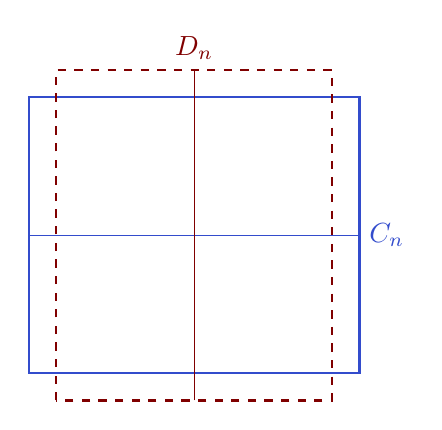
\begin{tikzpicture}[scale=0.7]
      \draw [thick, mblue] (0, 0) rectangle (6, 5);
      \draw [dashed, mred, thick] (0.5, -0.5) rectangle (5.5, 5.5);
      \node [right, mblue] at (6, 2.5) {$C_n$};
      \node [above, mred] at (3, 5.5) {$D_n$};
      \draw [mblue] (0, 2.5) -- (6, 2.5);
      \draw [mred] (3, -0.5) -- (3, 5.5);
    \end{tikzpicture}
  \end{center}
  Define $B_n$ to be the event that there is a top-bottom crossing of $D_n$ by closed edges of the dual.

  As before, it cannot be the case that $A_n$ and $B_n$ both occur. In fact, $A_n$ and $B_n$ partition the whole space, since if $A_n$ does not hold, then every path from left to right of $C_n$ is blocked by a closed path of the dual. Thus, we know
  \[
    \P(A_n) + \P(B_n) = 1.
  \]
  But also by symmetry, we have $\P(A_n) = \P(B_n)$. So
  \[
    \P (A_n) = \frac{1}{2}.
  \]
  On the other hand, for any point on the left edge, the probability of it reaching the right edge decays exponentially with $n$. Thus,
  \[
    \P(A_n) \leq n (n + 1) \P(0 \leftrightarrow \partial B_n) \leq (n + 1) e^{-cn}
  \]
  which is a contradiction. So we are done.
\end{proof}

So we now know that $p_c = \frac{1}{2}$. We now want to prove that
\[
  \P_{\frac{1}{2}}(0 \leftrightarrow \partial B(n)) \leq A n^{-\alpha}
\]
for some $A, \alpha$. To prove this, we again consider the dual lattice. Observe that if we have a closed dual circuit around the origin, then this prevents the existence of an open path from the origin to a point far far away. What we are going to do is to construct ``zones'' in the dual lattice like this:
\begin{center}
  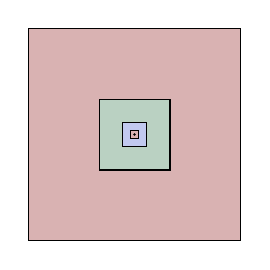
\begin{tikzpicture}[scale=0.1]
    \draw [fill=mred!30!white] (-13.5, -13.5) rectangle (13.5, 13.5);
    \draw [fill=mgreen!30!white] (-4.5, -4.5) rectangle (4.5, 4.5);
    \draw [fill=mblue!30!white] (-1.5, -1.5) rectangle (1.5, 1.5);
    \draw [fill=mred!30!white] (-0.5, -0.5) rectangle (0.5, 0.5);
    \node [fill, circle, inner sep = 0, minimum size = 1] at (0, 0) {};
  \end{tikzpicture}
\end{center}
The idea is to choose these zones in a way such that the probability that each zone contains a closed circuit around the origin is $\geq \zeta$ for some fixed $\zeta$. Thus, if $B(n)$ contains $m$ many of these zones, then the probability that $0$ is connected to $\partial B(n)$ is bounded above by $(1 - \zeta)^m$. We would then be done if we can show that $m \sim \log n$.

The main strategy to bounding these probabilities is to use FKG. For example, if we want to bound the probability that there is a closed circuit in a region
\begin{center}
  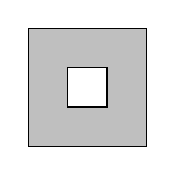
\begin{tikzpicture}
    \draw [fill=gray!50!white] (0, 0) rectangle (1.5, 1.5);
    \draw [fill=white] (0.5, 0.5) rectangle (1, 1);
  \end{tikzpicture}
\end{center}
then we cut it up into the pieces
\begin{center}
  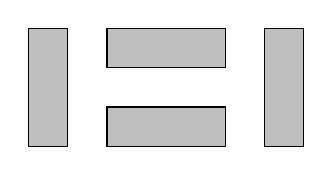
\begin{tikzpicture}
    \draw [fill=gray!50!white] (0, 0) rectangle (1.5, 0.5);
    \draw [fill=gray!50!white] (0, 1) rectangle (1.5, 1.5);

    \draw [fill=gray!50!white] (-1, 0) rectangle (-0.5, 1.5);
    \draw [fill=gray!50!white] (2, 0) rectangle (2.5, 1.5);
  \end{tikzpicture}
\end{center}
If we can bound the probability of there being a left-to-right crossing of a horizontal piece, and hence by symmetry the probability of there being a top-to-bottom crossing of a vertical piece, then FKG gives us a bound on the probability of there being a closed circuit.

For convenience of notation, we prove these bounds for open paths in the primal lattice. We make the following definitions:
\begin{align*}
  B(k\ell, \ell) &= [-\ell, (2k - 1)\ell] \times [-\ell, \ell]\\
  B(\ell) &= B(\ell, \ell) = [-\ell, \ell]^2\\
  A(\ell) &= B(3\ell) \setminus B(\ell)\\
  LR(k\ell ,\ell) &= \{\text{there exists left-right crossing of $B(k\ell, \ell)$ of open edges}\}\\
  LR(\ell) &= LR(\ell, \ell)\\
  O(\ell) &= \{\text{there exists open circuit in $A(\ell)$ that contains $0$ in its interior}\}.
\end{align*}
We first note that we have already proven the following:
\begin{prop}
  $\P_{\frac{1}{2}}(LR(\ell)) \geq \frac{1}{2}$ for all $\ell$.
\end{prop}

\begin{proof}
  We have already seen that the probability of there being a left-right crossing of $[0, n + 1] \times [0, n]$ is at least $\frac{1}{2}$. But if there is a left-right crossing of $[0, n + 1] \times [0, n]$, then there is also a left-right crossing of $[0, n] \times [0, n]$!
\end{proof}

For a general $p$, Russo--Symour--Welsh (RSW) lets us bound $\P_p(O(\ell))$ by $\P_p(LR(\ell))$:
\begin{thm}[Russo--Symour--Welsh (RSW) theorem]\index{Russo--Symour--Welsh}\index{RSW}
  If $\P_p(LR(\ell)) = \alpha$, then
  \[
    \P_p(O(\ell)) \geq \left(\alpha \left(1 - \sqrt{1 - \alpha}\right)^4\right)^{12}.
  \]
\end{thm}

A large part of the proof is done by the cut-and-paste argument we sketched above. However, to successfully do cut-and-paste, it turns out we need bounds on the probability of a left-right crossing on something that is \emph{not} a square. The key, non-trivial estimate is the following:
\begin{lemma}
  If $\P_p(LR(\ell)) = \alpha$, then
  \[
    \P_p\left(LR\left(\tfrac{3}{2}\ell, \ell\right)\right) \geq (1 - \sqrt{1 - \alpha})^3.
  \]
\end{lemma}

To prove this, we need a result from the first example sheet:
\begin{lemma}[$n$th root trick]\index{$n$th root trick}
  If $A_1, \ldots, A_n$ are increasing events all having the same probability, then
  \[
    \P_p(A_1) \geq 1 - \left(1 - \P_p\left(\bigcup_{i = 1}^n A_i\right)\right)^{1/n}.
  \]
\end{lemma}

\begin{proof}[Proof sketch]
  Observe that the proof of FKG works for \emph{decreasing} events as well, and then apply FKG to $A_i^c$.
\end{proof}

We can now prove our initial lemma.
\begin{proof}[Proof sketch]
  Let $\mathcal{A}$ be the set of left-right crossings of $B(\ell) = [-\ell, \ell]^2$. Define a partial order on $\mathcal{A}$ by $\pi_1 \leq \pi_2$ if $\pi_1$ is contained in the closed bounded region of $B(\ell)$ below $\pi_2$.

  Note that given any configuration, if the set of open left-right crossings is non-empty, then there exists a lowest one. Indeed, since $\mathcal{A}$ must be finite, it suffices to show that meets exist in this partial order, which is clear.

  For a left-right crossing $\pi$, let $(0, y_\pi)$ be the last vertex on the vertical axis where $\pi$ intersects, and let $\pi_r$ be the path of the path that connects $(0, y_\pi)$ to the right.
  \begin{center}
    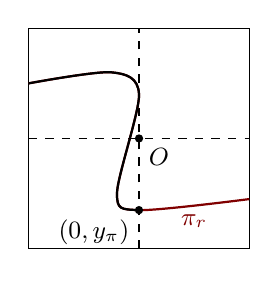
\begin{tikzpicture}[scale=0.7]

       \draw (-2, -2) rectangle (2, 2);
       \draw [dashed] (0, -2) -- (0, 2);
       \draw [dashed] (-2, 0) -- (2, 0);
       \node [circ] at (0, 0) {};
       \node [anchor = north west] {\small $O$};

       \draw [thick, mred] plot [smooth] coordinates {(-2, 1) (-0.5, 1.2) (0, 0.8) (-0.4, -1) (0, -1.3) (2, -1.1)};
       \begin{scope}
         \clip (-2, -2) -- (0, -2) -- (0, 0) -- (2, 0) -- (2, 2) -- (-2, 2) -- (-2, -2);
         \draw [thick, black] plot [smooth] coordinates {(-2, 1) (-0.5, 1.2) (0, 0.8) (-0.4, -1) (0, -1.3) (2, -1.1)};
       \end{scope}
       \node [circ] at (0, -1.3) {};
       \node [anchor = north east] at (0, -1.3) {\small$(0, y_\pi)$};
       \node [below, mred] at (1, -1.2) {\small$\pi_r$};
    \end{tikzpicture}
  \end{center}
  Let
  \begin{align*}
    \mathcal{A}_- &= \{\pi \in \mathcal{A}: y_\pi \leq 0\}\\
    \mathcal{A}_+ &= \{\pi \in \mathcal{A}: y_\pi \geq 0\}
  \end{align*}
   Letting $B(\ell)' = [0, 2\ell] \times [-\ell, \ell]$, our goal is to find a left-right crossing of the form
  \begin{center}
    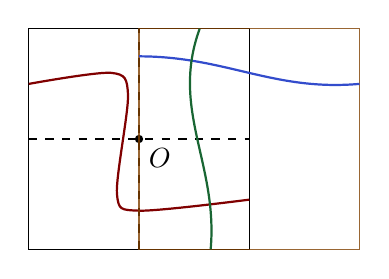
\begin{tikzpicture}[scale=0.7]
       \draw (-2, -2) rectangle (2, 2);
       \draw [dashed] (0, -2) -- (0, 2);
       \draw [dashed] (-2, 0) -- (2, 0);
       \node [circ] at (0, 0) {};
       \node [anchor = north west] {$O$};

       \draw [thick, mred] plot [smooth] coordinates {(-2, 1) (-0.5, 1.2) (-0.2, 0.8) (-0.4, -1) (0, -1.3) (2, -1.1)};

       \draw [morange!50!black, opacity=0.8] (0, -2) rectangle (4, 2);

       \draw [mblue, thick] (0, 1.5) edge [out=0, in=185] (4, 1);

       \draw [mgreen, thick] (1.1, 2) edge [out=250, in=85] (1.3, -2);
    \end{tikzpicture}
  \end{center}
  More precisely, we want the following paths:
  \begin{enumerate}
    \item Some $\pi \in \mathcal{A}_-$
    \item Some top-bottom crossing of $B(\ell')$ that crosses $\pi_r$.
    \item Some left-right crossing of $B(\ell')$ that starts at the positive (i.e.\ non-negative) $y$ axis.
  \end{enumerate}
  To understand the probabilities of these events happening, we consider the ``mirror'' events and then apply the square root trick.

  Let $\pi_r'$ be the reflection of $\pi_r$ on $\{(\ell, k): k \in \Z\}$. For any $\pi \in \mathcal{A}$, we define
  \begin{align*}
    V_\pi &= \{\text{all edges of $\pi$ are open}\}\\
    M_\pi &= \{\text{exists open crossing from top of $B(\ell)'$ to $\pi_r \cup \pi_r'$}\}\\
    M_\pi^- &= \{\text{exists open crossing from top of $B(\ell)'$ to $\pi_r$}\}\\
    M_\pi^+ &= \{\text{exists open crossing from top of $B(\ell)'$ to $\pi_r'$}\}\\\
    L^+ &= \{\text{exists open path in $\mathcal{A}_+$}\}\\
    L^- &= \{\text{exists open path in $\mathcal{A}_-$}\}\\
    L_\pi &= \{\text{$\pi$ is the lowest open LR crossing of $B(\ell)$}\}\\
    N &= \{\text{exists open LR crossing of $B(\ell)'$}\}\\
    N^+ &= \{\text{exists open LR crossing in $B(\ell)'$ starting from positive vertical axis}\}\\
    N^- &= \{\text{exists open LR crossing in $B(\ell)'$ starting from negative vertical axis}\}
  \end{align*}
  In this notation, our previous observation was that
  \[
    \underbrace{\bigcup_{\pi \in \mathcal{A}_-}(V_\pi \cap M_{\pi}^-)}_{G} \cap N^+ \subseteq LR\left(\frac{3}{2} \ell, \ell\right)
  \]
  So we know that
  \[
    \P_p\left(LR\left(\frac{3}{2}\ell, \ell\right)\right) \geq \P_p(G \cap N') \geq \P_p(G) \P_p(N^+),
  \]
  using FKG.

  Now by the ``square root trick'', we know
  \[
    \P_p(N^+) \geq 1 - \sqrt{1 - \P_p(N^+ \cup N^-)}.
  \]
  Of course, we have $\P_p(N^+ \cup N^-) = \P_p(LR(\ell)) = \alpha$. So we know that
  \[
    \P_p(N^+) \geq 1 - \sqrt{1 - \alpha}.
  \]
  We now have to understand $G$. To bound its probability, we try to bound it by the union of some disjoint events. We have
  \begin{align*}
    \P_p(G) &= \P_p\left(\bigcup_{\pi \in \mathcal{A}_-} (V_\pi \cap M_\pi^-)\right)\\
    &\geq \P_p\left(\bigcup_{\pi \in A_-} (M_\pi^- \cap L_\pi)\right)\\
    &= \sum_{\pi \in \mathcal{A}_-} \P_p(M_\pi^- \mid L_\pi) \P_p(L_\pi).
  \end{align*}
  \begin{claim}
    \[
      \P_p(M_\pi^- \mid L_\pi) \geq 1 - \sqrt{1 - \alpha}.
    \]
  \end{claim}
  Note that if $\pi$ intersects the vertical axis in one point, then $\P_p(M_\pi^- \mid L_\pi) = \P_p(M_\pi^- \mid V_\pi)$, since $L_\pi^-$ tells us what happens below $\pi$, and this does not affect the occurrence of $M_\pi^-$.

  Since $M_\pi^-$ and $V_\pi$ are increasing events, by FKG, we have
  \[
    \P_p(M_\pi^- \mid V_\pi) \geq \P_p(M_\pi^-) \geq 1 - \sqrt{1 - \P_p(M_\pi^- \cup M_\pi^+)} = 1 - \sqrt{1 - \P_p(M_\pi)}.
  \]
  Since $\P_p(M_\pi) \geq \P_p(LR(\ell)) = \alpha$, the claim follows.

  In the case where $\pi$ is more complicated, we will need an extra argument, which we will not provide.

  Finally, we have
  \[
    \P_p(G) \geq \sum_{\pi \in \mathcal{A}_-} \P_p(L_\pi) (1 - \sqrt{1 - \alpha}) = (1 - \sqrt{1 - \alpha})\P_p(L^-).
  \]
  But again by the square root trick,
  \[
    \P_p(L^-) \geq 1 - \sqrt{1 - \P_p(L^+ \cup L^-)} = 1 - \sqrt{1 - \alpha},
  \]
  and we are done.
\end{proof}

We now do the easy bit to finish off the theorem:
\begin{lemma}
  \begin{align*}
    \P_p(LR(2\ell ,\ell)) &\geq \P_p(LR(\ell)) \left(\P_p\left(LR\left(\frac{3}{2}\ell, \ell\right)\right)\right)^2\\
    \P_p(LR(3\ell ,\ell)) &\geq \P_p(LR(\ell)) \left(\P_p\left(LR\left(2\ell, \ell\right)\right)\right)^2\\
    \P_p(O(\ell)) &\geq \P_p(LR(3\ell, \ell))^4
  \end{align*}
\end{lemma}

\begin{proof}\leavevmode
  To prove the first inequality, consider the box $[0, 4\ell] \times [-\ell, \ell]$.
  \begin{center}
    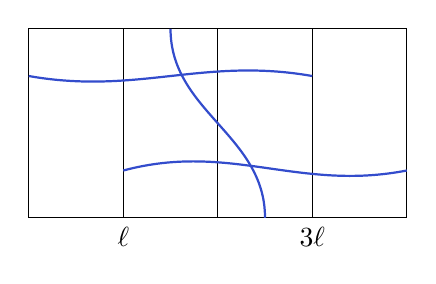
\begin{tikzpicture}[scale=0.6]
      \draw (0, 0) rectangle (2, 4);
      \draw (2, 0) rectangle (4, 4);
      \draw (4, 0) rectangle (6, 4);
      \draw (6, 0) rectangle (8, 4);
      \node [below] at (6, 0) {$3\ell$};
      \node [below] at (2, 0) {$\ell$};

      \draw [mblue, thick] (0, 3) edge [out=-10, in=170] (6, 3);
      \draw [mblue, thick] (2, 1) edge [out=15, in=191] (8, 1);
      \draw [mblue, thick] (3, 4) edge [out=270, in=90] (5, 0);
    \end{tikzpicture}
  \end{center}
  We let
  \begin{align*}
    LR_1 &= \{\text{exists left-right crossing of }[0, 3\ell] \times [-\ell, \ell]\}\\
    LR_2 &= \{\text{exists left-right crossing of }[\ell, 4\ell] \times [-\ell, \ell]\}\\
    TB_1 &= \{\text{exists top-bottom crossing of }[\ell, 3\ell] \times [-\ell, \ell]\}.
  \end{align*}
  Then by FKG, we find that
  \[
    \P_p(LR(2\ell, \ell)) \geq \P_p(LR_1 \cap LR_2 \cap TB_1) \geq \P_p(LR_1) \P_p(LR_2) \P_p(TB_1).
  \]
  The others are similar.
\end{proof}

\begin{thm}
  There exists positive constants $\alpha_1, \alpha_2, \alpha_3, \alpha_4, A_1, A_2, A_4$ such that
  \begin{align*}
    \P_{\frac{1}{2}} (0 \leftrightarrow \partial B(n)) &\leq A_1 n^{-\alpha_1}\\
    \P_{\frac{1}{2}} (|\mathcal{C}(0)| \geq n) &\leq A_2 n^{-\alpha_2}\\
    \E(|\mathcal{C}(0)|^{\alpha_3}) &\leq \infty
  \end{align*}
  Moreover, for $p > p_c = \frac{1}{2}$, we have
  \[
    \theta(p) \leq A_4 \left(p - \frac{1}{2}\right)^{\alpha_4}.
  \]
\end{thm}
It is an exercise on the example sheet to prove that $\P_{\frac{1}{2}}(0 \leftrightarrow B(n)) \geq \frac{1}{2\sqrt{n}}$ using the BK inequality. So the true decay of $\P_{\frac{1}{2}}(0 \leftrightarrow \partial B(n))$ is indeed a power law.

\begin{proof}\leavevmode
  \begin{enumerate}
    \item We first prove the first inequality. Define dual boxes
      \[
        B(k)_d = B(k) + \left(\frac{1}{2}, \frac{1}{2}\right).
      \]
      The dual annuli $A(\ell)_d$ are defined by
      \[
        A(\ell)_d = B(3\ell)_d \setminus B(\ell)_d.
      \]
      We let $O(\ell)_d$ be the event that there is a closed dual circuit in $A(\ell)_d$ containing $\left(\frac{1}{2}, \frac{1}{2}\right)$. Then RSW tells us there is some $\zeta \in (0, 1)$ such that
      \[
        \P_{\frac{1}{2}}(O(\ell)_d) \geq \zeta,
      \]
      independent of $\ell$. Then observe that
      \[
        \P_{\frac{1}{2}} (0 \leftrightarrow \partial B(3^k + 1)) \leq \P_p(O(3^r)_d\text{ does not occur for all }r < k).
      \]
      Since the annuli $(A(3^r)_d)$ are disjoint, the events above are independent. So
      \[
        \P_{\frac{1}{2}}(0 \leftrightarrow \partial B(3^k + 1)) \leq (1 - \zeta)^k,
      \]
      and this proves the first inequality.

    \item The second inequality follows from the first inequality plus the fact that $|\mathcal{C}(0)| \geq n$ implies $0 \leftrightarrow \partial B(g(n))$, for some function $g(n) \sim \sqrt{n}$.

    \item To show that $\E_{\frac{1}{2}}[|\mathcal{C}(0)|^{\alpha_3}] < \infty$ for some $\alpha_3$, we observe that this expectation is just
      \[
        \sum_n \P_{\frac{1}{2}}(|\mathcal{C}(0)|^{\alpha_3} \geq n).
      \]
    \item To prove the last part, note that
      \[
        \theta(p) = \P_p(|\mathcal{C}(0)| = \infty) \leq \P_p(0 \leftrightarrow \partial B_n)
      \]
      for all $n$. By the corollary of Russo's formula, and since $\{0 \leftrightarrow \partial B_n\}$ only depends on the edges in $B_n$, which are $\leq 18 n^2$, we get that
      \[
        \P_{\frac{1}{2}}(0 \leftrightarrow \partial B_n) \geq \left(\frac{1}{2p}\right)^{18n^2}\P_p(0 \leftrightarrow \partial B_n).
      \]
      So
      \[
        \theta(p) \leq (2p)^{18n^2} \P_{\frac{1}{2}}(0 \leftrightarrow \partial B_n) \leq A_1 (2p)^{18n^2} n^{-\alpha_1}.
      \]
      Now take $n = \lfloor (\log 2p)^{-1/2} \rfloor $. Then as $p \searrow \frac{1}{2}$, we have
      \[
        n \sim \frac{1}{(2p - 1)^{\frac{1}{2}}}.
      \]
      Substituting this in, we get
      \[
        \theta(p) \leq C \left(p - \frac{1}{2}\right)^{\alpha_1/2}.\qedhere
      \]%\qedhere
  \end{enumerate}
\end{proof}

By similar methods, we can prove that
\begin{thm}
  When $d = 2$ and $p > p_c$, there exists a positive constant $c$ such that
  \[
    \P_p(0 \leftrightarrow \partial B(n), |\mathcal{C}(0)| < \infty) \leq e^{-cn}.
  \]
\end{thm}

It is natural to ask if we have a similar result in higher dimensions. In higher dimensions, all the techniques in $\Z^2$ don't work.

\subsubsection*{Higher dimensions}

\index{slab percolation}In $d \geq 3$, define the \emph{slab}
\[
  S_k = \Z^2 \times \{0, 1, \ldots, k\}^{d - 2}.
\]
Then $S_k \subseteq S_{k + 1} \subseteq \Z^d$.

In general, for a graph $G$, we let $p_c(G)$ be the critical probability of bond percolation in $G$. Then we have
\[
  p_c(S_k) \geq p_c(S_{k + 1}) \geq p_c.
\]
So the sequence $(p_c(S_k))$ must converge to a limit. Call this limit\index{$p_c^{slab}$}
\[
  p_c^{slab} = \lim_{k \to \infty} p_c(S_k).
\]
We know that $p_c^{slab} \geq p_c$.

A lot of the results we can prove for $\Z^2$ can be proven for $p_c^{slab}$ instead of $p_c$. So the natural question is how $p_c^{slab}$ is related to $p_c$, and in particular, if they are equal. This has been an open question for a long time, until Grimmett and Marstrand proved it.

\begin{thm}[Grimmett--Marstrand]\index{Grimmett--Marstrand theorem}
  Let $F$ be an infinite-connected subset of $\Z^d$ with $p_c(F) < 1$. Then for all $\eta > 0$, there exists $k \in \N$ such that
  \[
    p_c(2k F + B_k) \leq p_c + \eta.
  \]
  In particular, for all $d \geq 3$, $p_c^{slab} = p_c$.
\end{thm}
We shall not prove the theorem, but we shall indicate how the ``in particular'' part works.

We take $F = \Z^2 \times \{0\}^{d - 2}$. Then
\[
  2kF + B_k = \Z^2 \times ([-k, k]^{d - 2} \cap \Z^{d - 2}),
\]
a translate of $S_{2k}$. So $p_c(S_{2k}) = p_c(2kF + B_k) \to p_c$ as $k \to \infty$.

A consequence of Grimmett-Marstrand is that
\begin{thm}
  If $d \geq 3$ and $p > p_c$, then there exists $c > 0$ such that
  \[
    \P_p(0 \leftrightarrow \partial B(n), |\mathcal{C}(0)| < \infty) \leq e^{-cn}.
  \]
\end{thm}

\subsection{Conformal invariance and SLE in \texorpdfstring{$d = 2$}{d = 2}}
Instead of working on $\Z^2$, we will now work on the triangular lattice $\T$. We consider \term{site percolation}. So every vertex is open (black) with probability $p$ and closed (white) with probability $1 - p$, independently for different vertices.

Like for $\Z^2$, we can show that $p = p_c(\T) = \frac{1}{2}$.

Let $D$ be an open simply connected domain in $\R^2$ with $\partial D$ a Jordan curve. Let $a, b, c \in \partial D$ be $3$ points labeled in anti-clockwise order. Consider the triangle $T$ with vertices $A = 0$, $B = 1$ and $C = e^{i\pi/3}$. By the Riemann mapping theorem, there exists a conformal map $\varphi: D \to T$ that maps $a \mapsto A$, $b \mapsto B$, $c \mapsto C$.

Moreover, this can be extended to $\partial D$ such that $\varphi: \bar{D} \to \bar{T}$ is a homeomorphism. If $x$ is in the arc $bc$, then it will be mapped to $X = \varphi(x)$ on the edge $BC$ of $T$.

Focus on the case $p = \frac{1}{2}$. We can again put a triangular lattice inside $D$, with mesh size $\delta$. We let $ac \leftrightarrow bx$ to mean the event that there is an open path in $D$ joining the arc $ac$ to $bx$.

Then by RSW (for $\T$), we get that
\[
  \P_\delta(ac \leftrightarrow bx) \geq c > 0,
\]
independent of $\delta$. We might ask what happens when $\delta \to 0$. In particular, does it converge, and what does it converge to?

Cardy, a physicist studying conformal field theories, conjectured that
\[
  \lim_{\delta \to 0} \P_\delta(ac \leftrightarrow bx) = |BX|.
\]
He didn't really write it this way, but expressed it in terms of hypergeometric functions. It was Carlesson who expressed it in this form.

In 2001, Smirnov proved this conjecture.

\begin{thm}[Smirnov, 2001]
  Suppose $(\Omega, a, b, c, d)$ and $(\Omega', a', b', c', d')$ are conformally equivalent. Then
  \[
    \P(ac \leftrightarrow bd\text{ in }\Omega) = \P(a' c' \leftrightarrow b' d'\text{ in }\Omega').
  \]
\end{thm}
This says percolation at criticality on the triangular lattice is conformally invariant.

We may also take the dual of the triangular lattice, which is the hexagonal lattice. Colour a hexagon black if the center is black, and similarly for whites. Suppose we impose the boundary condition on the upper half plane that the hexagons are black when $x > 0, y = 0$, and white when $x < 0, y = 0$.

Starting at $(x, y) = (0, 0)$, we explore the interface between the black and white by always keeping a black to our right and white on our right. We can again take the limit $\delta \to 0$. What is this exploration path going to look like in the limit $\delta \to 0$? It turns out this is an SLE(6) curve.

To prove this, we use the fact that the exploration curve satisfies the \emph{locality property}, namely that if we want to know where we will be in the next step, we only need to know where we currently are.

%Let $\gamma_t$ be a continuous curve in $\H$, and let $K_t$ be the unbounded component of $\H \setminus \gamma [0, t]$. Then there is a conformal map $g_t: \H \setminus K_t \to \H$ such that
%\[
%  \frac{\d}{\d t} g_t(x) = \frac{2}{g_t(z) - a(t)},
%\]
%and $a(t) = g_t(\gamma_t)$, $g_0(z) = z$.
%
%This is known as \term{Loewner's equation}.
%
%If we take $a(t) = \sqrt{\kappa} B_t$, where $B_t$ is a standard Brownian motion, this gives us SLE($\kappa$).

\section{Random walks}
\subsection{Random walks in finite graphs}
We shall consider weighted random walks on finite graphs. Let $G = (V, E)$ be a finite connected graph. We assign a conductances/weights to the edges $(c(e))_{e \in E}$. Here $c$ is a function of the edges, so we require $c(xy) = c(yx)$.

In the weighted random walk on $G$, the probability of going from $x$ to $y$ (assuming $x \sim y$) is
\[
  \P(x, y) = \frac{c(x, y)}{ c(x)},\quad c(x) = \sum_{z \sim x} c(x, z).
\]
If we put $c(e) = 1$ for all $e$, then this is just a simple random walk, with
\[
  \P(x, y) =
  \begin{cases}
    \frac{1}{\deg x} & y \sim x\\
    0 & \text{otherwise}
  \end{cases}.
\]
The weighted random walk is reversible with respect to $\pi(x) = \frac{c(x)}{c_G}$, where $c_G = \sum_x c(x)$, because
\[
  \pi(x) P(x, y) = \frac{c(x)}{c_G} \cdot \frac{c(x, y)}{c(x)} = \pi(y) \P(y, x).
\]
Conversely, every reversible Markov chain can be represented as a random walk on a weighted graph --- place an edge $\{x, y\}$ if $\P(x, y) > 0$. By reversibility, $\P(x, y) > 0$ iff $\P(y, x) = 0$. Define weights
\[
  c(x, y) = \pi(x) \P(x, y)
\]
for all $x \sim y$.

One way to understand random walks on weighted graphs is to think of them as currents in electrical networks. We set the resistance on the edges by
\[
  r(e) = \frac{1}{c(e)}.
\]
Naturally, we would like to talk about currents flowing through the circuit.
\begin{defi}[Flow]\index{flow}
  A \emph{flow} $\theta$ on $G$ is a function defined on oriented edges which is anti-symmetric, i.e.\ $\theta(x, y) = - \theta(y, x)$.
\end{defi}
Not every flow can be thought of as a current. We fix two distinguished vertices $a$ and $z$, called the \term{source} and the \term{sink} respectively. We think of current as entering the network through $a$ and exiting through $z$. Through any other vertex, the amount of current going in should equal the amount of current going out.

\begin{defi}[Divergence]\index{divergence}
  The \emph{divergence} of a flow $\theta$ is
  \[
    \div \theta (x) = \sum_{y \sim x} \theta(x, y).
  \]
\end{defi}
By the antisymmetry property, we have
\[
  \sum_x \div \theta(x) = \sum_x \sum_{y \sim x} \theta(x, y) = \sum_{x \sim y} \theta(x, y) = 0.
\]
\begin{defi}[Flow from $a$ to $z$]\index{flow}
  A flow $\theta$ from $a$ to $z$ is a flow such that
  \begin{enumerate}
    \item $\div \theta(x) = 0$ for all $x \not \in \{a, z\}$. \hfill (\term{Kirchhoff's node law})
    \item $\div \theta(a) \geq 0$.
  \end{enumerate}
  The \term{strength} of the flow from $a$ to $z$ is $\|\theta\| = \div \theta(a)$.\index{$\|\theta\|$}We say this is a \term{unit flow} if $\|\theta\| = 1$.
\end{defi}
Since $\sum \div \theta(x) = 0$, a flow from $a$ to $z$ satisfies $\div \theta(z) = - \div \theta(a)$.

Now if we believe in Ohm's law, then the voltage difference across each edge is $I(x, y) r(x, y)$. So we have
\[
  W(x) = W(y) + r(x, y) I(x, y)
\]
for all $y$. We know that if we sum $I(x, y)$ over all $y$, then the result vanishes. So we rewrite this as
\[
  c(x, y) W(x) = c(x, y) W(y) + I(x, y).
\]
Summing over all $y$, we find that the voltage satisfies
\[
  W(x) = \sum_{x \sim y} \frac{c(x, y)}{c(x)} W(y) = \sum_{x \sim y} \P(x, y) W(y).
\]
\begin{defi}[Harmonic function]\index{harmonic function}
  Let $P$ be a transition matrix on $\Omega$. We call $h$ \emph{harmonic} for $P$ at the vertex $x$ if
  \[
    h(x) = \sum_y \P(x, y) h(y).
  \]
\end{defi}

We now take this as a \emph{definition} of what a voltage is.
\begin{defi}[Voltage]\index{voltage}
  A \emph{voltage} $W$ is a function on $\Omega$ that is harmonic on $\Omega \setminus \{a, z\}$.
\end{defi}

The first theorem to prove is that given any two values $W(a)$ and $W(z)$, we can find a unique voltage with the prescribed values at $a$ and $z$.

More generally, if $B \subseteq \Omega$, and $X$ is a Markov chain with matrix $P$, then we write
\[
  \tau_B = \min\{t \geq 0: X_t \in B\},
\]

\begin{prop}
  Let $P$ be an irreducible matrix on $\Omega$ and $B \subseteq \Omega$, $f: B \to \R$ a function. Then
  \[
    h(x) = \E_x [f(X_{\tau_B})]
  \]
  is the unique extension of $f$ which is harmonic on $\Omega \setminus B$.
\end{prop}

\begin{proof}
  It is obvious that $h(x) = f(x)$ for $x \in B$. Let $x \not\in B$. Then
  \begin{align*}
    h(x) &= \E_x [f(X_{\tau_B})] \\
    &= \sum_y \P(x, y) \E_x[f(X_{\tau_B}) \mid X_1 = y]\\
    &= \sum_y \P(x, y) \E_y[f(X_{\tau_B})]\\
    &= \sum_Y \P(x, y) h(y)
  \end{align*}
  So $h$ is harmonic.

  To show uniqueness, suppose $h'$ be another harmonic extension. Take $g = h - h'$. Then $g = 0$ on $B$. Set
  \[
    A = \left\{x: g(x) = \max_{y \in \Omega \setminus B} g(y) \right\},
  \]
  and let $x \in A \setminus B$. Now since $g(x)$ is the weighted average of its neighbours, and $g(y) \leq g(x)$ for all neighbours $y$ of $x$, it must be the case that $g(x) = g(y)$ for all neighbours of $y$.

  Since we assumed $G$ is connected, we can construct a path from $x$ to the boundary, where $g$ vanishes. So $g(x) = 0$. In other words, $\max g = 0$. Similarly, $\min g = 0$. So $g = 0$.
\end{proof}

Given a voltage, Ohm's law\index{Ohm's law} defines a natural flow, called the \emph{current flow}.
\begin{defi}[Current flow]\index{current flow}
  The \emph{current flow} associated to the voltage $W$ is
  \[
    I(x, y) = \frac{W(x) - W(y)}{r(x, y)} = c(x, y) (W(x) - W(y)).
  \]
\end{defi}
The current flow has an extra property, namely that it satisfies the \term{cycle law}. For any cycle $e_1, e_2, \ldots, e_n$, we have
\[
  \sum_{i = 1}^n r(e_i) I (e_i) = 0.
\]

\begin{prop}
  Let $\theta$ be a flow from $a$ to $z$ satisfying the cycle law for any cycle. Let $I$ the current flow associated to a voltage $W$. If $\|\theta\| = \|I\|$, then $\theta = I$.
\end{prop}

\begin{proof}
  Take $f = \theta - I$. Then $f$ is a flow which satisfies Kirchhoff's node law at all vertices and the cycle law for any cycle. We want to show that $f = 0$. Suppose not. The we can find some $e_1$ such that $f(e_i) > 0$. But
  \[
    \sum_{y\sim x} f(x, y) = 0
  \]
  for all $x$, so there must exist an edge $e_2$ that $e_1$ leads to such that $f(e_2) > 0$. Continuing this way, we will get a cycle of ordered edges where $f > 0$, which violates the cycle law.
\end{proof}
Let $W_0$ be a voltage with $W_0(a) = 1$ and $W_0(z) = 0$, and let $I_0$ be the current associated to $W_0$. Then any other voltage $W$ can be written as
\[
  W(x) = (W(a) - W(z)) W_0(x) + W(z).
\]
So, noting that $W_0(a) = 1$, we have
\[
  W(a) = W(x) = (W(a) - W(z))(W_0(a) - W_0(x)).
\]
Thus, if $I$ is the current associated to $W$, then
\[
  \|I\| = \sum_{x \sim a} I(a, x) = \sum_{x \sim a} \frac{W(a) - W(x)}{r(a, x)} = (W(a) - W(z)) \|I_0\|.
\]
So we know that
\[
  \frac{W(a) - W(z)}{\|I\|} = \frac{1}{\|I_0\|},
\]
and in particular does not depend on $W$.

\begin{defi}[Effective resistance]\index{Effective resistance}
  The \emph{effective resistance} $R_{\mathrm{eff}}(a, z)$ of an electric network is defined to be the ratio
  \[
    R_{\mathrm{eff}}(a, z) = \frac{W(a) - W(z)}{\|I\|}
  \]
  for any voltage $W$ with associated current $I$. The \term{effective conductance} is $C_{\mathrm{eff}}(a, z) = R_{\mathrm{eff}}(a, z)^{-1}$.
\end{defi}

\begin{prop}
  Take a weighted random walk on $G$. Then
  \[
    \P_a(\tau_z < \tau_a^+) = \frac{1}{c(a) R_{\mathrm{eff}}(a, z)},
  \]
  where $\tau_a^+ = \min \{t \geq 1: X_t = a\}$.
\end{prop}

\begin{proof}
  Let
  \[
    f(x) = \P_x(\tau_z < \tau_a).
  \]
  Then $f(a) = 0$ and $f(z) = 1$. Moreover, $f$ is harmonic on $\Omega \setminus \{a, z\}$. Let $W$ be a voltage. By uniqueness, we know
  \[
    f(x) = \frac{W(a) - W(x)}{W(a) - W(z)}.
  \]
  So we know
  \begin{align*}
    \P_a(\tau_z < \tau_a^+) &= \sum_{x \sim a} \P(a, x) f(x) \\
    &= \sum_{x \sim a} \frac{c(a, x)}{c(a)} \frac{W(a) - W(x)}{W(a) - W(z)}\\
    &= \frac{1}{c(a) (W(a) - W(z))} \sum_{x \sim a}I(a, x)\\
    &= \frac{\|I\|}{c(a) (W(a) - W(z))}\\
    &= \frac{1}{c(a) R_{\mathrm{eff}}(a, z)}.\qedhere
  \end{align*}
\end{proof}

\begin{defi}[Green kernel]\index{Green kernel}
  Let $\tau$ be a stopping time. We define the \emph{Green kernel} to be
  \[
    G_\tau(a, x) = \E_a \left[ \sum_{t = 0}^\infty \mathbf{1}(X_t = x, t < \tau)\right].
  \]
\end{defi}
This is the expected number of times we hit $x$ before $\tau$ occurs.
\begin{cor}
  For any reversible chain and all $a, z$, we have
  \[
    G_{\tau_z}(a, a) = c(a) R_{\mathrm{eff}}(a, z).
  \]
\end{cor}

\begin{proof}
  By the Markov property, the number of visits to $a$ starting from $a$ until $\tau_z$ is the geometric distribution $Geo(\P_a(\tau_z < \tau_a^+))$. So
  \[
    G_{\tau_z}(a, a) = \frac{1}{\P_a(\tau_z < \tau_a^+)} = c(a) R_{\mathrm{eff}}(a, z).\qedhere
  \]
\end{proof}

Practically, to compute the effective resistance, it is useful to know some high school physics. For example, we know that conductances in parallel add:
\begin{center}
  \begin{tikzpicture}
    \draw (0, 0) -- (1, 0) -- (1, 0.5) -- (2, 0.5);
    \draw (1, 0) -- (1, -0.5) -- (2, -0.5);
    \draw [decorate, decoration={zigzag}] (2, 0.5) -- (2.5, 0.5) node [pos=0.5, above] {$c_1$};
    \draw [decorate, decoration={zigzag}] (2, -0.5) -- (2.5, -0.5) node [pos=0.5, below] {$c_2$};

    \draw (2.5, 0.5) -- (3.5, 0.5) -- (3.5, -0.5) -- (2.5, - 0.5);
    \draw (3.5, 0) -- (4.5, 0);

    \node at (5.5, 0) {$=$};

    \draw (6.5, 0) -- (7.5, 0);
    \draw [decorate, decoration={zigzag}] (7.5, 0) -- (8, 0) node [pos=0.5, above] {$c_1 + c_2$};
    \draw (8, 0) -- (9, 0);
  \end{tikzpicture}
\end{center}

Thus, if $e_1$ and $e_2$ are two edges with the same endvertices, then we we can replace them by a single edge of conductance the sum of the conductances. We can prove that this actually works by observing that the voltages and currents remain unchanged outside of $e_1, e_2$, and we check that Kirchhoff's and Ohm's law are satisfied with
\[
  I(e) = I(e_1) + I(e_2).
\]
Similarly, resistances in series add. Let $v$ be a node of degree $2$ and let $v_1$ and $v_2$ be its $2$ neighbours. Then we can replace these $2$ edges by a single edge of resistance $r_1 + r_2$. Again, to justify this, we check Kirchoff's and Ohm's law with
\[
  I(v_1 v_2) = I(v_1 v) + I(vv_2).
\]
\begin{center}
  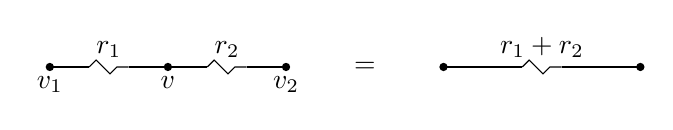
\begin{tikzpicture}
    \draw (0, 0) -- (0.5, 0);
    \draw [decorate, decoration={zigzag}] (0.5, 0) -- (1, 0) node [pos=0.5, above] {$r_1$};
    \draw (1, 0) -- (2, 0);
    \draw [decorate, decoration={zigzag}] (2, 0) -- (2.5, 0) node [pos=0.5, above] {$r_2$};
    \draw (2.5, 0) -- (3, 0);

    \node [below] at (0, 0) {$v_1$};
    \node [below] at (1.5, 0) {$v$};
    \node [below] at (3, 0) {$v_2$};

    \node [circ] at (0, 0) {};
    \node [circ] at (1.5, 0) {};
    \node [circ] at (3, 0) {};

    \node at (4, 0) {$=$};
    \draw (5, 0) -- (6, 0);
    \draw [decorate, decoration={zigzag}] (6, 0) -- (6.5, 0) node [pos=0.5, above] {$r_1 + r_2$};
    \draw (6.5, 0) -- (7.5, 0);
    \node [circ] at (5, 0) {};
    \node [circ] at (7.5, 0) {};
  \end{tikzpicture}
\end{center}

We can also glue $2$ vertices of the same potential, keeping all other edges. Current and potential are unchanged since current doesn't flow if there is the same potential.

\begin{ex}
  Let $T$ be a finite connected tree, and $a, z$ two vertices. Then $R_{\mathrm{eff}}(a, z)$ is the graph distance between $a$ and $z$.
\end{ex}

It turns out it is not convenient to work with our definition of effective resistance. Instead, we can use the well known result from high school physics $P = IV = I^2 R$. For any flow, we define

\begin{defi}[Energy]\index{energy}
  Let $\theta$ be a flow on $G$ with conductances $(c(e))$. Then the \emph{energy} is
  \[
    \mathcal{E}(\theta) = \sum_e (\theta(e))^2 r(e).
  \]
  Here we sum over unoriented edges.
\end{defi}
Note that given any flow, we can always increase the energy by pumping more and more current along a cycle. Thus, we might expect the lowest energy configuration to be given by the flows satisfying the cycle law, and if we focus on unit flows, the following should not be surprising:

\begin{thm}[Thomson's principle]\index{Thomson's principle}
  Let $G$ be a finite connected graph with conductances $(c(e))$. Then for any $a, z$, we have
  \[
    R_{\mathrm{eff}}(a, z) = \inf \{\mathcal{E}(\theta): \text{$\theta$ is a unit flow from $a$ to $z$}\}.
  \]
  Moreover, the unit current flow from $a$ to $z$ is the unique minimizer.
\end{thm}

\begin{proof}
  Let $i$ be the unit current flow associated to potential $\varphi$. Let $j$ be another unit flow $a \to z$. We need to show that $\mathcal{E}(j) \geq \mathcal{E}(i)$ with equality iff $j = i$.

  Let $k = j - i$. Then $k$ is a flow of $0$ strength. We have
  \[
    \mathcal{E}(j) = \mathcal{E}(i + k) = \sum_e (i(e) + k(e))^2 r(e) = \mathcal{E}(i) + \mathcal{E}(k) + 2 \sum_e i(e) k(e) r(e).
  \]
  It suffices to show that the last sum is zero. By definition, we have
  \[
    i(x, y) = \frac{\varphi(x) - \varphi(y)}{r(x, y)}.
  \]
  So we know
  \begin{align*}
    \sum_e i(e) k(e) r(e) &= \frac{1}{2} \sum_x \sum_{y \sim x} (\varphi(x) - \varphi(y)) k(x, y)\\
    &= \frac{1}{2} \sum_x \sum_{y \sim x} \varphi(x)k(x, y) + \frac{1}{2} \sum_x \sum_{y \sim x} \varphi(x) k(x, y).
  \end{align*}
  Now note that $\sum_{y \sim x} k(x, y) = 0$ for any $x$ since $k$ has zero strength. So this vanishes.

  Thus, we get
  \[
    \mathcal{E}(j) = \mathcal{E}(i) + \mathcal{E}(k),
  \]
  and so $\mathcal{E}(j) \geq \mathcal{E}(i)$ with equality iff $\mathcal{E}(k) = 0$, i.e.\ $k(e) = 0$ for all $e$.
\end{proof}
Using this characterization, it is then immediate that
\begin{thm}[Rayleigh's monotonicity principle]\index{Rayleigh's monotonicity principle}\index{monotonicity principle}
  Let $G$ be a finite connected graph and $(r(e))_e$ and $(r'(e))_e$ two sets of resistances on the edges such that $r(e) \leq r'(e)$ for all $e$. Then
  \[
    R_{\mathrm{eff}}(a, z; r) \leq R_{\mathrm{eff}}(a, z; r').
  \]
  for all $a, z \in G$.
\end{thm}

\begin{proof}
  By definition of energy, for any current $i$, we have
  \[
    \mathcal{E}(i; r) \leq \mathcal{E}(i; r').
  \]
  Then take the infimum and conclude by Thompson.
\end{proof}

\begin{cor}
  Suppose we add an edge to $G$ which is not adjacent to $a$. This increases the escape probability
  \[
    \P_a(\tau_z < \tau_a^+).
  \]
\end{cor}

\begin{proof}
  We have
  \[
    \P_a(\tau_z < \tau_z^+) = \frac{1}{c(a) R_{\mathrm{eff}}(a, z)}.
  \]
  We can think of the new edge as an edge having infinite resistance in the old graph. By decreasing it to a finite number, we decrease $R_{\mathrm{eff}}$.
\end{proof}

\begin{defi}[Edge cutset]\index{edge cutset}\index{cutset}
  A set of edges $\Pi$ is an edge-cutset separating $a$ from $z$ if every path from $a$ to $z$ uses an edge of $\Pi$.
\end{defi}

\begin{thm}[Nash--Williams inequality]\index{Nash--Williams inequality}
  Let $(\Pi_k)$ be disjoint edge-cutsets separating $a$ from $z$. Then
  \[
    R_{\mathrm{eff}}(a, z) \geq \sum_k \left(\sum_{e \in \Pi_k}c(e)\right)^{-1}.
  \]
\end{thm}
The idea is that if we combine all paths in each $\Pi_k$ to a single path with conductance $\sum_{e \in \Pi_k} c(e)$, then every path has to use all of these edges, so we can bound the effective resistance.

\begin{proof}
  By Thompson, it suffices to prove that for any unit flow $\theta$ from $a$ to $z$, we have
  \[
    \sum_e (\theta(e))^2 r(e) \geq \sum_k \left(\sum_{e \in \Pi_k}c(e)\right)^{-1}.
  \]
  Certainly, we have
  \[
    \sum_e (\theta(e))^2 r(e) \geq \sum_k \sum_{e \in \Pi_k}(\theta(e))^2 r(e).
  \]
  We now use Cauchy--Schwarz to say
  \begin{align*}
    \left(\sum_{e \in \Pi_k} (\theta(e))^2 r(e)\right) \left(\sum_{e \in \Pi_k}c(e)\right) &\geq \left(\sum_{e \in \Pi_k} |\theta(e)| \sqrt{r(e) c(e)} \right)^2\\
    &= \left(\sum_{e \in \Pi_k} |\theta(e)|\right)^2.
  \end{align*}
  The result follows if we show that the final sum is $\geq 1$.

  Let $F$ be the component of $G \setminus \Pi_k$ containing $a$. Let $F'$ be the set of all edges that start in $F$ and land outside $F$. Then we have
  \[
    1 = \sum_{x \in F} \div \theta(x) \leq \sum_{e \in F'} |\theta(e)| \leq \sum_{e \in \Pi_k} |\theta(e)|.\qedhere
  \]
\end{proof}

\begin{cor}
  Consider $B_n = [1, n]^2 \cap \Z^2$. Then
  \[
    R_{\mathrm{eff}}(a, z) \geq \frac{1}{2} \log (n - 1).
  \]
\end{cor}
There is also an upper bound of the form $R_{\mathrm{eff}}(a, z) \leq c \log n$. So this is indeed the correct order. The proof involves constructing an explicit flow with this energy.

\begin{proof}
  Take
  \[
    \Pi_k = \{(v, u) \in B_n: \|v\|_\infty = k - 1, \|u\|_\infty = k\}.
  \]
  Then
  \[
    |\Pi_k| = 2(k - 1),
  \]
  and so
  \[
    R_{eff}(a, z) \geq \sum_{k = 1}^{ - 1} \frac{1}{|\Pi_k|} \geq \frac{1}{2} \log (n - 1).\qedhere
  \]
\end{proof}

We shall need the following result:
\begin{prop}
  Let $X$ be an irreducible Markov chain on a finite state space. Let $\tau$ be a stopping time such that $\P_a(X_\tau = a) = 1$ and $\E_a[\tau] < \infty$ for some $a$ in the state space. Then
  \[
    G_\tau(a, x) = \pi(x) \E_a[\tau].
  \]
\end{prop}
A special case of this result was proven in IB Markov Chain, where $\tau$ was taken to be the first return time to $a$. The proof of this is very similar, and we shall not repeat it.

Using this, we can prove the commute-time identity.
\begin{thm}[Commute time identity]\index{commute time identity}
  Let $X$ be a reversible Markov chain on a finite state space. Then for all $a, b$, we have
  \[
    \E_a [\tau_b] + \E_b[ \tau_a] = c(G) R_{\mathrm{eff}}(a, b),
  \]
  where
  \[
    c(G) = 2 \sum_e c(e).
  \]
\end{thm}

\begin{proof}
  Let $\tau_{a,b}$ be the first time we hit $a$ after we hit $b$. Then $\P_a(X_{\tau_{a, b}} = a) = 1$. By the proposition, we have
  \[
    G_{\tau_{a, b}}(a, a) = \pi(a) \E_a[\tau_{a,b}].
  \]
  Since starting from $a$, the number of times we come back to $A$ by $\tau_{a, b}$ is the same as up to time $\tau_b$, we get
  \[
    G_{\tau_{a,b}}(a, a) = G_{\tau_b}(a, a) = c(a) R_{\mathrm{eff}}(a, b).
  \]
  Combining the two, we get
  \[
    \pi(a) \E_a[\tau_{a, b}] = c(a) R_{\mathrm{eff}}(a, b).
  \]
  Thus, the result follows.
\end{proof}
In particular, from the commute-time identity, we see that the effective resistance satisfies the triangle inequality, and hence defines a metric on any graph.

\subsection{Infinite graphs}
Finally, let's think a bit about how we can develop the same theory for infinite graphs.

Let $G$ be an infinite connected weighted graph with conductances $(c(e))_e$. Let $0$ be a distinguished vertex. Let $(G_k = (V_k, E_k))_k$ be an \term{exhaustion} of $G$ by finite graphs, i.e.
\begin{itemize}
  \item $V_k \subseteq V_{k + 1}$ for all $k$;
  \item $0 \in V_k$ for all $k$;
  \item $\bigcup_k V_k = V$;
  \item $E_k$ is the set of edges of $E$ with both end points in $V_k$.
\end{itemize}

Let $G_n^*$ be the graph obtained by gluing all the vertices of $V \setminus V_n$ into a single point $z_n$ and setting
\[
  c(x, z_n) = \sum_{z \in V \setminus V_n} c(x, z)
\]
for all $x \in V_n$. Now observe that $R_{\mathrm{eff}}(0, z_n; G_n^*)$ is a non-decreasing function of $n$ (Rayleigh). So the limit as $n \to \infty$ exists. We set \index{$R_{\mathrm{eff}}(0, \infty)$}
\[
  R_{\mathrm{eff}}(0, \infty) = \lim_{n \to \infty} R_{\mathrm{eff}}(0, z_n; G_n*).
\]
This is independent of the choice of exhaustion by Rayleigh. % or by interlacing.

Now we have
\[
  \P_0(\tau_0^+ = \infty) = \lim_{n \to \infty} \P_0(\tau_{z_n} < \tau_0^+) = \frac{1}{c(0) R_{\mathrm{eff}}(0, z_n; G_n^*)} = \frac{1}{c(0) R_{\mathrm{eff}}(0, \infty)}.
\]
\begin{defi}[Flow]\index{flow}
  Let $G$ be an infinite graph. A \emph{flow} $\theta$ from $0$ to $\infty$ is an anti-symmetric function on the edges such that $\div \theta(x) = 0$ for all $x \not= 0$.
\end{defi}

\begin{thm}
  Let $G$ be an infinite connected graph with conductances $(c(e))_e$. Then
  \begin{enumerate}
    \item Random walk on $G$ is recurrent iff $R_{\mathrm{eff}}(0, \infty) = \infty$.
    \item The random walk is transient iff there exists a unit flow $i$ from $0$ to $\infty$ of finite energy
      \[
        \mathcal{E}(i) = \sum_e (i(e))^2 r(e).
      \]
  \end{enumerate}
\end{thm}

\begin{proof}
  The first part is immediate since
  \[
    \P_0(\tau_0^+ = \infty) = \frac{1}{c(0) R_{\mathrm{eff}}(0, \infty)}.
  \]
  To prove the second part, let $\theta$ be a unit flow from $0$ to $\infty$ of finite energy. We want to show that the effective resistance is finite, and it suffices to extend Thompson's principle to infinite graphs.

  Let $i_n$ be the unit current flow from $0$ to $z_n$ in $G_n^*$. Let $v_n(x)$ be the associated potential. Then by Thompson,
  \[
    R_{\mathrm{eff}}(0, z_n; G_n^*) = \mathcal{E}(i_n).
  \]
  Let $\theta_n$ be the restriction of $\theta$ to $G_n^*$. Then this is a unit flow on $G_n^*$ from $0$ to $z_n$. By Thompson, we have
  \[
    \mathcal{E}(i_n) \leq \mathcal{E}(\theta_n) \leq \mathcal{E}(\theta) < \infty.
  \]
  So
  \[
    R_{\mathrm{eff}}(0, \infty) = \lim_{n \to \infty} \mathcal{E}(i_n).
  \]
  So by the first part, the flow is transient.

  Conversely, if the random walk is transient, we want to construct a unit flow from $0$ to $\infty$ of finite energy. The idea is to define it to be the limit of $(i_n)(x, y)$.

  By the first part, we know $R_{\mathrm{eff}}(0, \infty) = \lim \mathcal{E}(i_n) < \infty$. So there exists $M > 0$ such that $\mathcal{E}(i_n) \leq M$ for all $n$. Starting from $0$, let $Y_n(x)$ be the number of visits to $x$ up to time $\tau_{z_n}$. Let $Y(x)$ be the total number of visits to $x$. Then $Y_n(x) \nearrow Y(x)$ as $n \to \infty$ almost surely.

  By monotone convergence, we get that
  \[
    \E_0[Y_n(x)] \nearrow \E_0[Y(x)] < \infty,
  \]
  since the walk is transient. On the other hand, we know
  \[
    E_0[Y_n(x)] = G_{\tau_{z_n}}(0, x).
  \]
  It is then easy to check that $\frac{G_{\tau_{z_n}}(0, x)}{c(x)}$ is a harmonic function outside of $0$ and $z_n$ with value $0$ at $z_n$. So it has to be equal to the voltage $v_n(x)$. So
  \[
    v_n(x) = \frac{G_{\tau_{z_n}}(0, x)}{c(x)}.
  \]
  Therefore there exists a function $v$ such that
  \[
    \lim_{n \to \infty} c(x) v_n(x) = c(x) v(x).
  \]
  We define
  \[
    i(x, y) = c(x, y) (v(x) - v(y)) = \lim_{n \to \infty} c(x, y) (v_n(x) - v_n(y)) = \lim_{n \to \infty} i_n(x, y).
  \]
  Then by dominated convergence, we know $\mathcal{E}(i) \leq M$, and also $i$ is a flow from $0$ to $\infty$.
\end{proof}

Note that this connection with electrical networks only works for reversible Markov chains.

\begin{cor}
  Let $G' \subseteq G$ be connected graphs.
  \begin{enumerate}
    \item If a random walk on $G$ is recurrent, then so is random walk on $G'$.
    \item If random walk on $G'$ is transient, so is random walk on $G$.
  \end{enumerate}
\end{cor}

\begin{thm}[Polya's theorem]\index{Polya's theorem}
  Random walk on $\Z^2$ is recurrent and transient on $\Z^d$ for $d \geq 3$.
\end{thm}

\begin{proof}[Proof sketch]
  For $d = 2$, if we glue all vertices at distance $n$ from $0$, then
  \[
    R_{\mathrm{eff}}(0, \infty) \geq \sum_{i = 1}^{n - 1} \frac{1}{8i - 4} \geq c \cdot \log n
  \]
  using the parallel and series laws. So $R_{\mathrm{eff}}(0, \infty) = \infty$. So we are recurrent.

  For $d = 3$, we can construct a flow as follows --- let $S$ be the sphere of radius $\frac{1}{4}$ centered at the origin. Given any edge $\mathbf{e}$, take the unit square centered at the midpoint $\mathbf{m}_e$ of $\mathbf{e}$ and has normal $\mathbf{e}$. We define $|\theta(\mathbf{e})|$ to be the area of the radial projection on the sphere, with positive sign iff $\bra \mathbf{m}_e, \mathbf{e} \ket > 0$.

  One checks that $\theta$ satisfies Kirchoff's node law outside of $0$. Then we find that
  \[
    \mathcal{E}(\theta) \leq C \sum_n n^2 \cdot \left(\frac{1}{n^2}\right)^2 < \infty,
  \]
  since there are $\sim n^2$ edges at distance $n$, and the flow has magnitude $\sim \frac{1}{n^2}$.
\end{proof}

\begin{proof}[Another proof sketch]
  We consider a binary tree $T_\rho$ with edges joining generation to $n + 1$ having resistance $\rho^n$ for $\rho$ to be determined. Then
  \[
    R_{\mathrm{eff}}(T_\rho) = \sum_{n = 1}^\infty \left(\frac{\rho}{2}\right)^n,
  \]
  and this is finite when $\rho < 2$.

  Now we want to embed this in $\Z^3$ in such a way that neighbours in $T_\rho$ of generation $n$ and $n + 1$ are separated by a path of length of order $\rho^n$. In generation $n$ of $T_\rho$, there are $2^n$ vertices. On the other hand, the number of vertices at distance $n$ in $\Z^3$ will be of order $(\rho^n)^2$. So we need $(\rho^n)^2 \geq 2^n$. So we need $\rho > \sqrt{2}$. We can then check that
  \[
    R_{\mathrm{eff}}(0, \infty; \Z^3) \leq c \cdot R_{\mathrm{eff}}(T_\rho) < \infty.\qedhere
  \]
\end{proof}
Note that this method is rather robust. We only need to be able to embed our $T_\rho$ into $\Z^3$. Using a similar method, Grimmett, Kesten and Zhang (1993) showed that simple random walk on a supercritical bond percolation is transient for $d \geq 3$.

\section{Uniform spanning trees}
\subsection{Finite uniform spanning trees}
The relation between uniform spanning trees and electrical networks was discovered by Kirchoff in 1850's. Of course, he was not interested in uniform spanning tress, but in electrical networks themselves. One of the theorems we will prove is
\begin{thm}[Foster's theorem]\index{Foster's theorem}
  Let $G = (V, E)$ be a finite weighted graph on $n$ vertices. Then
  \[
    \sum_{e \in E}R_{\mathrm{eff}}(e) = n - 1.
  \]
\end{thm}
We can prove this using the commute-time formula, but there is a one-line proof using this connection between electrical networks and uniform spanning trees.
\begin{defi}[Spanning tree]\index{spanning tree}
  Let $G = (V, E)$ be a finite connected graph. A \emph{spanning tree} $T$ of $G$ is a connected subgraph of $G$ which is a tree\index{tree} (i.e.\ there are no cycles) and contains all the vertices in $G$.
\end{defi}

Let $\mathcal{T}$ be the set of all spanning trees of $G$. Pick $T \in \mathcal{T}$ uniformly at random. We call it the \term{uniform spanning tree}. We shall prove the following theorem:
\begin{thm}
  Let $e \not= f \in E$. Then
  \[
    \P(e \in T \mid f \in T) \leq \P(e \in T).
  \]
\end{thm}
It is tempting to ask a very similar question --- if we instead considered all spanning \emph{forests}, do we get the same result? Intuitively, we should, but it turns out this is an open question. So let's think about trees instead.

In order to prove this, we need the following result:
\begin{thm}[Kirchoff]
  Let $T$ be a uniform spanning tree, $e$ an edge. Then
  \[
    \P(e \in T) = R_{\mathrm{eff}}(e)
  \]
\end{thm}
Of course, this immediately implies Foster's theorem, since every tree has $n - 1$ edges.

\begin{notation}
  Fix two vertices $s, t$ of $G$. For all every edge $e = (a, b)$, define $\mathcal{N}(s, a, b, t)$ to be the set of spanning tress of $G$ whose unique path from $s$ to $t$ passes along the edge $(a, b)$ in the direction from $a$ to $b$. Write
  \[
    N(s, a, b, t) = |\mathcal{N}(s, a, b, t)|,
  \]
  and $N$ the total number of spanning trees.
\end{notation}

\begin{thm}
  Define, for every edge $e = (a, b)$,
  \[
    i(a, b) = \frac{N(s, a, b, t) - N(s, b, a, t)}{N}.
  \]
  Then $i$ is a unit flow from $s$ to $t$ satisfying Kirchoff's node law and the cycle law.
\end{thm}
Note that from the expression for $i$, we know that
\[
  i(a, b) = \P(T \in \mathcal{N}(s, a, b, t)) - \P(T \in \mathcal{N}(s, b, a, t)).
\]
\begin{proof}
  We first show that $i$ is a flow from $s$ to $t$. It is clear that $i$ is anti-symmetric. To check Kirchoff's node law, pick $a \not \in \{s, t\}$. We need to show that
  \[
    \sum_{x \sim a} i(a, x) = 0.
  \]
  To show this, we count how much each spanning tree contributes to the sum. In each spanning tree, the unique path from $s$ to $t$ may or may not contain $a$. If it does not contain $a$, it contributes $0$. If it contains $A$, then there is one edge entering $a$ and one edge leaving $a$, and it also contributes $0$. So every spanning tree contributes exactly zero to the sum.

  So we have to prove that $i$ satisfies the cycle law. Let $C = (v_1, v_2, \ldots, v_{n + 1} = v_1)$ be a cycle. We need to show that
  \[
    \sum_{i = 1}^n i(v_i, v_{i + 1}) = 0.
  \]
  To prove this, it is easier to work with ``bushes'' instead of trees. An \term{$s/t$ bush} is a forest that consists of exactly $2$ trees, $T_s$ and $T_t$, such that $s \in T_s$ and $t \in T_t$. Let $e = (a, b)$ be an edge. Define $\mathcal{B}(s, a, b, t)$ to be the set of $s/t$ bushes such that $a \in T_s$ and $b \in T_t$.

  We claim that $|\mathcal{B}(s, a, b, t)| = N(s, a, b, t)$. Indeed, given a bush in $\mathcal{B}(s, a, b, t)$, we can add the edge $e = (a, b)$ to get a spanning tree whose unique path from $s$ to $t$ passes through $e$, and vice versa.

  Instead of considering the contribution of each tree to the sum, we count the contribution of each bush to the set. Then this is easy. Let
  \begin{align*}
    F_+ &= |\{(v_j, v_{j + 1}): B \in \mathcal{B}(s, v_j, v_{j + 1}, t)\}\\
    F_- &= |\{(v_j, v_{j + 1}): B \in \mathcal{B}(s, v_{j + 1}, v_j, t)\}
  \end{align*}
  Then the contribution of $B$ is
  \[
    \frac{F_+ - F_-}{N}.
  \]
  By staring it at long enough, since we have a cycle, we realize that we must have $F_+ = F_-$. So we are done.

  Finally, we need to show that $i$ is a unit flow. In other words,
  \[
    \sum_{x \sim s} i(s, x) = 1.
  \]
  But this is clear, since each spanning tree contributes $\frac{1}{N}$ to $i(s, x)$, and there are $N$ spanning trees.
\end{proof}

We can now prove the theorem we wanted to prove.
\begin{thm}
  Let $e \not= f \in E$. Then
  \[
    \P(e \in T \mid f \in T) \leq \P(e \in T).
  \]
\end{thm}

\begin{proof}
  Define the new graph $G.f$ to be the graph obtained by gluing both endpoints of $f$ to a single vertex (keeping multiple edges if necessary). This gives a correspondence between spanning trees of $G$ containing $f$ and spanning trees of $G.f$. But
  \[
    \P(e \in T \mid f \in T) = \frac{\text{number of spanning trees of $G.f$ containing $e$}}{\text{number of spanning trees of $G.f$}}.
  \]
  But this is just $\P(e \in \text{UST of $G.f$})$, and this is just $R_{\mathrm{eff}}(e; G .f)$. So it suffices to show that
  \[
    R_{\mathrm{eff}}(e; G.f) \leq R_{\mathrm{eff}}(e; G).
  \]
  But this is clear by Rayleigh's monotone principle, since contracting $f$ is the same as setting the resistance of the edge to $0$.
\end{proof}

In practice, how can we generate a uniform spanning tree? One way to do so is \term{Wilson's method}.

\begin{defi}[Loop erasure]\index{loop erasure}
  Let $x = \bra x_1, \ldots x_n\ket$ be a finite path in the graph $G$. We define the \emph{loop erasure} as follows: for any pair $i < j$ such that $x_i = x_j$, remove $x_{i + 1}, x_{i+2}, \ldots, x_j$, and keep repeating until no such pairs exist.
\end{defi}

To implement Wilson's algorithm, distinguish a root vertex of $G$, called $r$, and take an ordering of $V$. Set $T_0 = \{r\}$. Define $T_i$ inductively as follows: take the first vertex in the ordering is not in $T_i$. We start a simple random walk from this vertex, and run until it hits $T_i$, and erase the loops. Then set $T_{i + 1}$ to be the union of $T_i$ with this (loop-erased) path. Repeat until all vertices are used.

\begin{thm}[Wilson]
  The resulting tree is a uniform spanning tree.
\end{thm}
Note that in particular, the choice of ordering is irrelevant to the resulting distribution.

To prove this theorem, it is convenient to have a good model of how the simple random walk on $G$ is generated. Under any vertex $G$, place an infinite number of cards that contain iid instructions, i.e.\ each card tells us to which neighbour we jump. Different vertices have independent stacks. Whenever we are at a vertex $x$, look at the top card underneath it and go to the neighbour it instructs. Then throw away the top card and continue.

Given stacks of cards under the vertices of the graph, by revealing the top card of each vertex, we get a directed graph, where directed edges are of the form $(x, y)$, where $y$ is the instruction on the top card under $x$.

If there is no directed cycle, then we stop, and we have obtained a spanning tree. If there is a directed cycle, then we remove the top cards from all vertices on the cycle. We call this procedure \term{cycle popping}. Then we look at the top cards again and remove cycles and cards used.

We first prove a \emph{deterministic} lemma about cycle popping.
\begin{lemma}
  The order in which cycles are popped is irrelevant, in the sense that either the popping will never stop, or the same set of cycles will be popped, thus leaving the same spanning tree lying underneath.
\end{lemma}

\begin{proof}
  Given an edge $(x, S_x^i)$, where $S_x^i$ is the $i$th instruction under $x$, colour $(x, S_x^i)$ with colour $i$. A colour is now coloured, but not necessarily with the same colour.

  Suppose $C$ is a cycle that can be popped in the order $C_1, C_2, \ldots, C_n$, with $C_n = C$. Let $C'$ be any cycle in the original directed graph. We claim that either $C'$ does not intersect $C_1, \ldots, C_n$, or $C' = C_k$ for some $k$, and $C'$ does not intersect $C_1, \ldots C_{k - 1}$. Indeed, if they intersect, let $x \in C' \cap C_k$, where $k$ is the smallest index where they intersect. Then the edge coming out of $x$ will have colour $1$. Then $S_x^1$ is also in the intersection of $C'$ and $C_k$, and so the same is true for the edge coming out of $S_x^1$. Continuing this, we see that we must have $C_k = C'$. So popping $C_k, C_1, \ldots, C_{k - 1}, C_{k + 1}, \ldots, C_n$ gives the same result as popping $C_1, \ldots, C_n$.

  Thus, by induction, if $C$ is a cycle that is popped, then after performing a finite number of pops, $C$ is still a cycle that can be popped. So either there is an infinite number of cycles that can be popped, so popping can never stop, or every cycle that can be popped will be popped, thus in this case giving the same spanning tree.
\end{proof}

Using this, we can prove that Wilson's method gives the correct distribution. In Wilson's algorithm, we pop cycles by erasing loops in the order of cycle creation. This procedure will stop will probability $1$. With this procedure, we will reveal a finite set of coloured cycles $O$ lying over a spanning tree. Let $X$ be the set of all $(O, T)$, where $O$ is the set of coloured cycles lying on top of $T$, which arise from running the random walks.

Now if we can get to $(O, T)$, then we could also get to $(O, T')$ for any other spanning spanning tree $T'$, since there is no restriction on what could be under the stacks. So we can write
\[
  X = X_1 \times X_2,
\]
where $X_1$ is a certain set of finite sets of coloured cycles, and $X_2$ is the set of all spanning trees.

Define a function $\Psi$ on the set of cycles by
\[
  \Psi(C) = \prod_{e \in C} p(e),\quad p(e) = \frac{c(e)}{c(e_-)},
\]
where $e = (e_-, e_+)$, and $c(e_-)$ is the sum of the conductances of all edges with vertex $e_-$.

More generally, if $O$ is a set of cycles, then we write
\[
  \Psi(O) = \prod_{C \in O} \Psi(C).
\]
Then
\[
  \P(\text{get $(O, T)$ using Wilson's algorithm}) = \prod_{e \in \bigcup_{C \in O} C \cup T)} p(e) = \Psi(O) \cdot \Psi(T).
\]
Since this probability factorizes, it follows that the distribution of $O$ is independent of $T$, and the probability of getting $T$ is proportional to $\Psi(T)$. So $T$ has the distribution of a uniform spanning tree.

\begin{cor}[Cayley's formula]\index{Cayley's formula}
  The number of labeled unrooted trees on $n$-vertices is equal to $n^{n - 2}$.
\end{cor}

\begin{proof}
  Exercise.
\end{proof}

How can we generalize Wilson's algorithm to infinite graphs? If the graph is recurrent, then we can still use the same algorithm, and with probability one, the algorithm terminates. If we have a transient graph, then we can still perform the same algorithm, but it is not clear what the resulting object will be.

The \term{Aldous--Broder algorithm} is another way of generating a uniform spanning tree. Run a random walk that visits all vertices at least once. For every vertex other than the root, take the edge the walk crossed the first time it visited the vertex, and keep the edge in the spanning tree. It is an exercise to prove that this does give a uniform spanning tree. Again, this algorithm works only on a recurrent graph. A generalization to transient graphs was found by Hutchcroft.

\subsection{Infinite uniform spanning trees and forests}
Since recurrent graphs are boring, let $G$ be an infinite transient graph. Then a ``naive'' way to define a uniform spanning tree is by exhaustions.

Let $G_n$ be an exhaustion of $G$ by finite graphs. Define $G_n^W$ (where $W$ stands for ``wired'') to be the graph $G_n$, where all of the vertices of $G \setminus G_n$ are glued to a single vertex $z_n$. The ``free'' $G_n$ is just $G_n$ considered as a subgraph. It turns out the wired one is much easier to study.

Let $\mu_n$ be the uniform spanning tree measure on $G_n^W$. Let $B$ be a finite set of edges $B = \{e_1, \ldots, e_n\}$. Then for $T$ a UST of $G_n^W$, we have
\begin{align*}
  \mu_n(B \subseteq T) &= \prod_{k = 1}^m \mu(e_k \in T \mid e_j \in T\text{for all }j < k) \\
  &= \prod_{k = 1}^n R_{\mathrm{eff}}(e_k; G_n^W/\{e_j: j < k\}),
\end{align*}
where $G_n^W/\{e_j: j < k\}$ is the graph obtained from $G_n^W$ by contracting the edges $\{e_j: j < k\}$.

We want to show that $\mu_n$ as a sequence of measures converges. So we want to understand how $R_{\mathrm{eff}}(e_k; G_n^W/\{e_j: j < k\})$ changes when we replace $n$ with $n + 1$. By Rayleigh's monotonicity principle, since $G_n^W$ can be obtained from $G_{n + 1}^W$ by contracting more edges, we know the effective resistance increases when we replace $n$ with $n + 1$. So we know that
\[
  \mu_n(B \subseteq T) \leq \mu_{n + 1}(B \subseteq T).
\]
So $(\mu_n(B \subseteq T))$ is an increasing sequence. So we can define
\[
  \mu(B \subseteq \mathcal{F}) = \lim_{n \to \infty} \mu_n(B \subseteq T),
\]
and $\mathcal{F}$ is our uniform forest. We can then extend the definition of $\mu$ to cylinder events
\[
  \{\mathcal{F}: B_1 \subseteq \mathcal{F}, B_2 \cap \mathcal{F} = \emptyset\}
\]
with $B_1, B_2$ finite sets of edges, using inclusion-exclusion:
\[
  \mu(B_1 \subseteq \mathcal{F}, B_2 \cap \mathcal{F} = \emptyset) = \sum_{S \subseteq B_2} \mu(B_1 \cup S \subseteq \mathcal{F}) (-1)^{|S|}.
\]
Then by commuting limits, we find that in fact
\[
  \mu(B_1 \subseteq \mathcal{F}, B_2 \cap \mathcal{F} = \emptyset) = \lim_{n \to \infty} \mu_n (B_1 \subseteq T, B_2 \cap T = \emptyset).
\]
If $\mathcal{A}$ is a finite union or intersection of cylinder sets of this form, then we have
\[
  \mu(\mathcal{A}) = \lim_{n \to \infty} \mu_n(\mathcal{A}).
\]
So this gives a consistent family of measures.

By Kolmogorov's theorem, we get a unique probability measure $\mu$ supported on the forests of $G$. $\mu$ is called the \term{wired uniform spanning forest}. One can also consider the \term{free uniform spanning forest}, where we do the same thing but without gluing, however, this is more complicated and we will not study it.

We can adapt Wilson's algorithm to generate uniform spanning forests. This is called \term{Wilson's method rooted at infinity} (BKPS, 2001).

Let $G$ be a transient graph, and start with $\mathcal{F}_0 = \emptyset$. Pick an ordering of the vertices of $V = \{x_1, x_2, \ldots\}$. Inductively, from $x_n$, we start a simple random walk until the first time it hits $\mathcal{F}_{n - 1}$ if it does. If it doesn't, then run indefinitely. Call this (possibly infinite) path $\mathcal{P}_n$. Since $G$ is transient, $\mathcal{P}_n$ will visit every vertex finitely many times with probability $1$. So it makes sense to define the loop erasure of $\mathcal{P}_n$. Call it $LE(\mathcal{P}_n)$. We set
\[
  \mathcal{F}_n = \mathcal{F}_{n - 1} \cup LE(\mathcal{P}_n),
\]
and take
\[
  \mathcal{F} = \bigcup_n \mathcal{F}_n.
\]
As before, the order of $V$ that we take does not affect the final distribution.
\begin{prop}
  Let $G$ be a transient graph. The wired uniform spanning forest is the same as the spanning forest generated using Wilson's method rooted at infinity.
\end{prop}

\begin{proof}
  Let $e_1, \ldots, e_M$ be a finite set of edges. Let $T(n)$ be the uniform spanning tree on $G_n^W$. Let $\mathcal{F}$ be the limiting law of $T(n)$. Look at $G_n^W$ and generate $T(n)$ using Wilson's method rooted at $z_n$. Start the random walks from $u_1, u_2, \ldots, u_L$ in this order, where $(u_i)$ are all the end points of the $e_1, \ldots, e_M$ ($L$ could be less than $2M$ if the edges share end points).

  Start the first walk from $u_1$ and wait until it hits $z_n$; Then start from the next vertex and wait until it hits the previous path. We use the same infinite path to generate all the walks, i.e.\ for all $i$, let $(X_k(u_i))_{k \geq 0}$ be a simple random walk on $G$ started from $u_i$. When considering $G_n^W$, we stop these walks when they exit $G_n$, .e.\ if they hit $z_n$. In this way, we couple all walks together and all the spanning trees.

  Let $\tau_i^n$ be the first time the $i$th walk hits the tree the previous $i - 1$ walks have generated in $G_n^W$. Now
  \[
    \P(e_1, \ldots, e_M \in T(n)) = \P\left(e_1, \ldots, e_M \in \bigcup_{j = 1}^L LE(X_k(u_j)) : k \leq \tau_{j^n} \right).
  \]
  Let $\tau_j$ be the stopping times corresponding to Wilson's method rooted at infinity. By induction on $j$, we have $\tau_j^n \to \tau_j$ as $n \to \infty$, and by transience, we have $LE(X_k(u_j): k \leq \tau_j^k) \to LE(X_k(u_j): k \leq \tau_j)$. So we are done.
\end{proof}

\begin{thm}[Pemantle, 1991]
  The uniform spanning forest on $\Z^d$ is a single tree almost surely if and only if $d \leq 4$.
\end{thm}

Note that the above proposition tells us
\begin{prop}[Pemantle]
  The uniform spanning forest is a single tree iff starting from every vertex, a simple random walk intersects an independent loop erased random walk infinitely many times with probability $1$. Moreover, the probability that $x$ and $y$ are in the same tree of the uniform spanning forest is equal to the probability that simple random walk started from $x$ intersects an independent loop-erased random walk started from $y$.
\end{prop}

To further simplify the theorem, we use the following theorem of Lyons, Peres and Schramm:
\begin{thm}[Lyons, Peres, Schramm]
  Two independent simple random walks intersect infinitely often with probability $1$ if one walks intersects the loop erasure of the other one infinitely often with probability $1$.
\end{thm}

Using these, we can now prove the theorem we wanted. Note that proving things about intersection, rather than collisions, tends to be higher, because any attempts to, say, define the first intersection time would inherently introduce an asymmetry.

We prove half of Pemantle's theorem.
\begin{thm}
  The uniform spanning forest is not a tree for $d \geq 5$ with probability $1$.
\end{thm}

\begin{proof}[Proof of Pemantle's theorem]
  Let $X, Y$ be two independent simple random walks in $\Z^d$. Write
  \[
    I = \sum_{t = 0}^\infty \sum_{s = 0}^\infty \mathbf{1}(X_t = Y_s).
  \]
  Then we have
  \[
    \E_{x, y}[I] = \sum_t \sum_s \P_{x - y} (X_{t + s} = 0) \approx \sum_{t = \|x - y\|} t \P_{x - y}(X_t = 0).
  \]
  It is an elementary exercise to show that
  \[
    \P_x(X_t = 0) \leq \frac{c}{t^{d/2}},
  \]
  so
  \[
    \P_x(X_t = 0) \leq \sum_{t = \|x - y\|} \frac{1}{t^{d/2 - 1}}.
  \]
  For $d \geq 5$, for all $\varepsilon > 0$, we take $x, y$ such that
  \[
    \E_{x, y} [I] < \varepsilon.
  \]
  Then
  \[
    \P(\text{USF is connected}) \leq \P_{x, y}(I > 0) \leq \E_{x, y}[I] < \varepsilon.
  \]
  Since this is true for every $\varepsilon$, it follows that $\P(\text{USF is connected}) = 0$.
\end{proof}

\printindex
\end{document}
